\chapter{Convección Mixta en Flujos Completamente Desarrollados} \label{cap:desarrollado}
%\chapterquote{¡Lo viejo funciona, Juan!}{Alberto ``Tano'' Favalli}

El propósito de este capítulo es analizar, vía simulaciones numéricas, el flujo turbulento completamente desarrollado y asistido por fuerzas boyantes, en un canal vertical de placas paralelas. Para esto se utilizaron simulaciones DNS que cubren un extenso espectro de números de Reynolds, Richardson y Prandtl, lo que permite examinar la evolución desde convección forzada hasta convección natural. Tras describir los casos y las variables adimensionales de referencia, se presentan (i) magnitudes estadísticas de primer y segundo orden, (ii) la influencia del número de Prandtl sobre las subcapas viscosa y térmica, (iii) el número de Nusselt y (iv) el factor de fricción de Darcy.

En primer lugar, se analizan cantidades de primer y segundo orden, entre ellas los perfiles de velocidad y temperatura. Se observa que la fuerza boyante transforma los perfiles de velocidad hacia una morfología tipo “M” y desplaza el máximo de $\langle u_x^* \rangle$ hacia la pared. Luego, para flujos con $0 < \text{Ri}_b < 1$, los perfiles de temperatura adimensional se ubican por encima del caso puramente forzado y para $\text{Ri}_b>1$, la mezcla inducida por la flotación “aplana” el perfil medio adimensional de temperatura. En cuanto al número de Prandtl, su efecto se refleja en la ley de pared de temperatura: con $\text{Pr}=0\text{.}071$ se verifica $\langle \theta^{*} \rangle \simeq \text{Pr} \hspace{1mm} y^+$ hasta $y^+ \approx 30$, mientras que con $\text{Pr}=0\text{.}71$ concluye en $y^+ \approx 7$, lo que evidencia la influencia de $\text{Pr}$ en la capa conductiva. 

En segundo lugar, se abordan magnitudes de interés en ingeniería: el número de Nusselt y el factor de fricción de Darcy. Existe un intervalo $10^{-6} \lesssim \text{Bo} \lesssim 3\times10^{-5}$ (donde Bo es el número de boyancia \cite{jackson1989studies}) en el que $\text{Nu}$ se reduce respecto al caso puramente forzado; fuera de éste, la transferencia térmica se recupera y supera a la correspondiente de la convección forzada. Esta caída coincide con una disminución en la producción de turbulencia cerca de la pared. Por último, debido a la asistencia de la boyancia, el gradiente de velocidad en la pared aumenta y eleva el factor de fricción de Darcy. Además, se propone una correlación del mismo en función del número de boyancia (Bo) y se observa que reproduce con buena fidelidad tanto los datos simulados como los de referencia.


\newpage

\section{Casos simulados} 

Los resultados de las simulaciones realizadas en este capítulo corresponden a un flujo completamente desarrollado tanto térmica como hidrodinámicamente. Se emplearon Re$_o$=2100, 3150, 4278, 5000; Pr=0.071, 0.71; y valores de Richardson en el rango 0.04 $\lesssim$ Ri$_b$ $\lesssim$ 106. Para una simple conceptualización física, la variación de estos números adimensionales puede interpretarse de la siguiente manera: un aumento del número de Reynolds corresponde a un aumento del caudal; un incremento del número de Prandtl señala una reducción de la conductividad térmica; mientras que un mayor número de Richardson denota un crecimiento en el flujo de calor.

A modo de visualizar el tipo de simulaciones realizadas en este trabajo, en la Figura \ref{fig:map_flow_regime} se expone un ``mapa''  del régimen de flujo en función del número de Reynolds \textit{bulk}\footnote{Número de Reynolds basado en la velocidad \textit{bulk} y el diámetro hidráulico: $\text{Re}^D_b = 8/3 \hspace*{1mm} \text{Re}_o$} y el número de Richardson \textit{bulk}\footnote{Número de Richardson basado en la velocidad \textit{bulk} y el ancho del canal: $\text{Ri}_b = 9/2 \hspace*{1mm} \text{Ri}_o$}. Esta figura, que también muestra las simulaciones realizadas en este trabajo, supone que la convección natural no afecta la turbulencia del flujo y por tanto es indicativa, a priori, del tipo de flujos que caracterizarán nuestras simulaciones. Aceptando provisionalmente que la fuerza boyante no afecta la turbulencia del flujo, y tomando como referencia el diagrama de Moody \cite{white}, se presenta lo siguiente:



\begin{itemize}
	\item para valores de Re$^D_b$ $<$ 2000 el régimen es laminar,
	\item si 2000 $\lesssim$ Re$^D_b$ $\lesssim$ 4000 el régimen es de transición,
	\item y si Re$^D_b>$ 4000 el régimen es turbulento.
\end{itemize}
Por otra parte, el fenómeno de convección es \cite{incropera,cengelheat}:

\begin{itemize}
	\item forzado si Ri$_b<$ 0.1,
	\item mixto si 0.1 $<$ Ri$_b$ $<$ 10,
	\item y natural si Ri$_b$ $>$ 10.
\end{itemize}

Las simulaciones consideradas operan en régimen turbulento, con énfasis en convección mixta, incorporando casos donde predomina la convección forzada y otras donde predomina la convección natural. Este rango de parámetros constituye el marco para el análisis y la discusión del problema en las secciones siguientes.

\newpage

\begin{figure}[H]
  \centering
    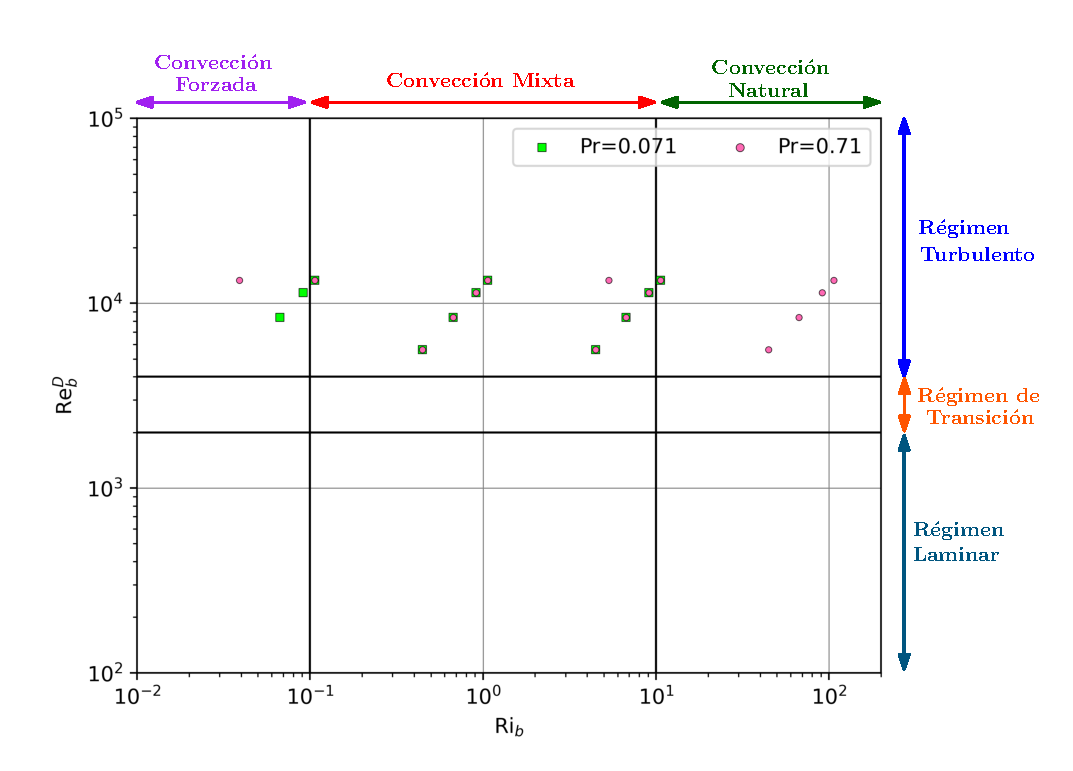
\includegraphics[width=0.8\textwidth]{figures/cap5/map.eps}
  \caption{Mapa de regímenes en el plano $Re^D_b$–$Ri_b$. Se señalan las zonas laminar, de transición y turbulenta, así como los dominios de convección forzada, mixta y natural.}
  \label{fig:map_flow_regime}
\end{figure}

\section{Magnitudes de Primer y Segundo Orden}

En esta sección se analiza la influencia de la fuerza boyante en las magnitudes estadísticas de primer y segundo orden. Para tal fin y por simplicidad, se considera únicamente el caso Re$_o$=5000 y Pr=0.71. Si el lector lo requiere, puede ver el Apéndice \ref{apen:desarrollado}, donde se encuentran disponibles los perfiles de dichas cantidades para el resto de números adimensionales considerados.

Como se menciona anteriormente, un aumento de Ri$_b$ (o un aumento de la fuerza boyante) denota un crecimiento en el flujo de calor. Esto puede interpretarse como un incremento de la energía térmica que se le entrega al sistema a través de las paredes cuando el flujo es ascendente\footnote{También es equivalente a quitarle energía térmica (enfriar las paredes) cuando la dirección del flujo es descendente.}.

\subsection{Perfiles de velocidad y de temperatura} \label{sec:velo_temp}

En la Figura \ref{fig:ux-Re5000-Pr071} se presentan los perfiles medios de velocidad  \textit{streamwise}\footnote{Es decir, en la dirección de la corriente.} para distintos números de Richardson. En dichos perfiles pueden distinguirse con claridad los tres regímenes de convección. Conforme se intensifica la fuerza boyante, las curvas adoptan una forma en ``M'', en concordancia con lo reportado por otros autores \cite{you2003direct, zhou2024direct}. A diferencia de la convección puramente forzada, el máximo de velocidad deja de ubicarse en la línea central del canal. Al aumentar $\mathrm{Ri}_b$, ese máximo migra hacia la pared y el perfil desarrolla dos picos locales, en lugar del único pico característico del régimen forzado \cite{carr1973velocity,steiner1971reverse,zhou2024direct}. Este comportamiento puede interpretarse cualitativamente del siguiente modo: en las proximidades de la pared el fluido se encuentra a mayor temperatura lo que implica menor densidad; en consecuencia, la fuerza boyante acelera el flujo en esa región y, por conservación de masa, el fluido ubicado en la zona central experimenta una desaceleración.

\begin{figure}[H]
  \centering
  \subfloat[]{
    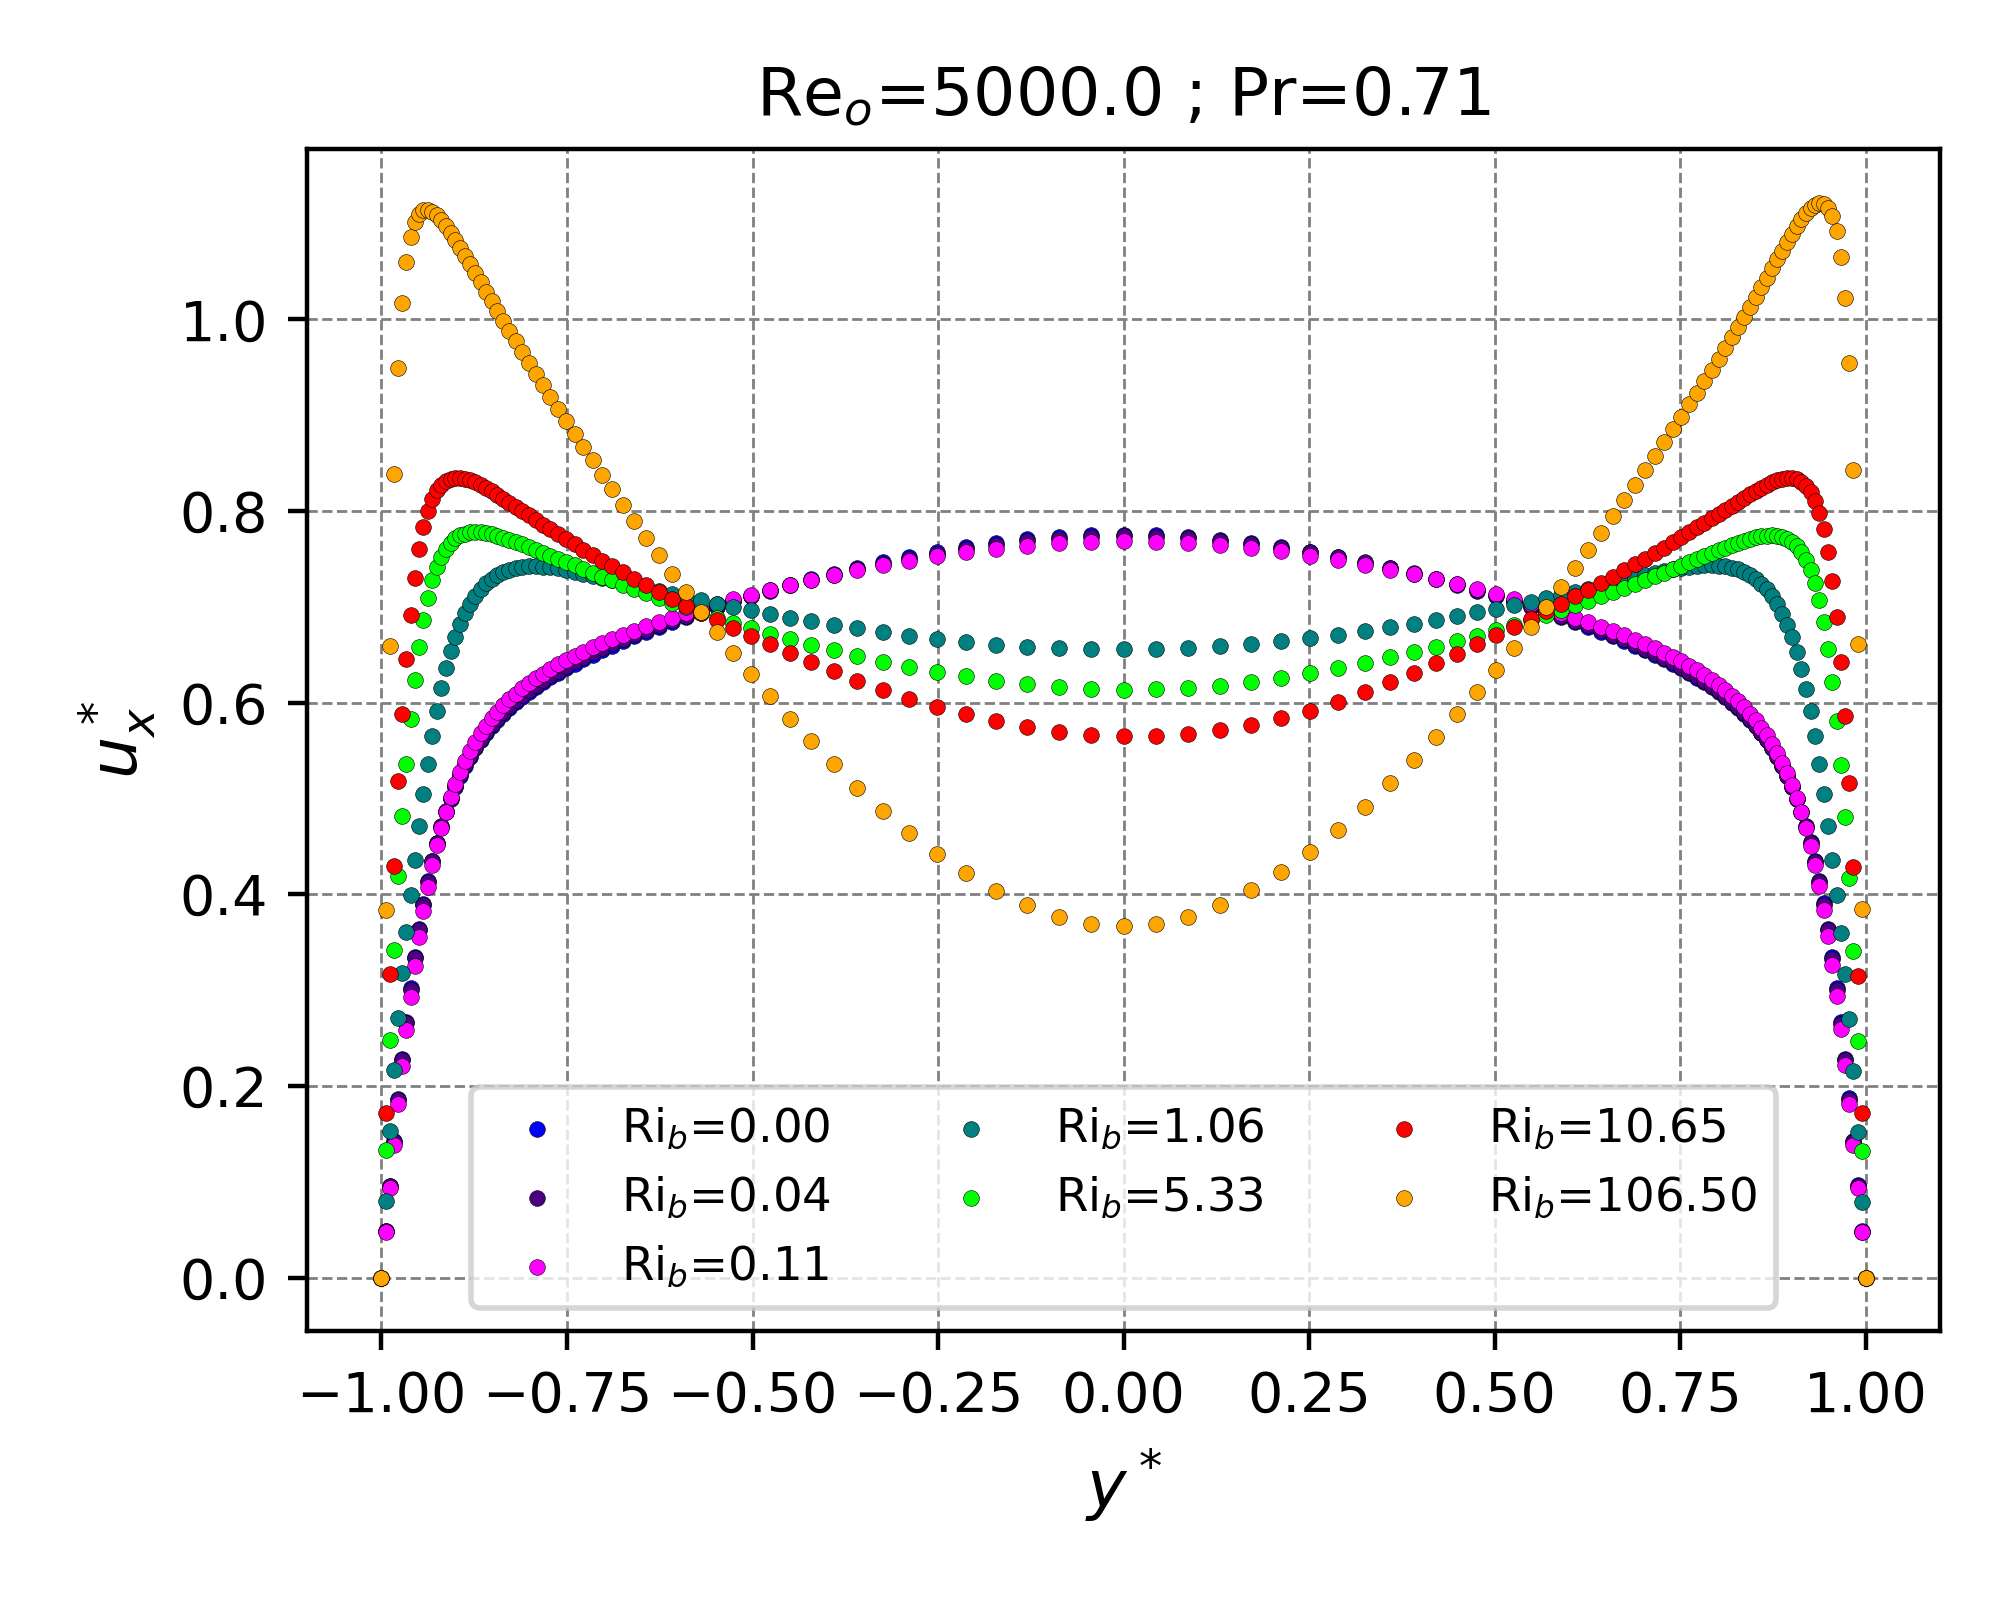
\includegraphics[width=0.49\textwidth]{figures/cap5/Re5000-Pr071/ux_mean_profile.png}
    	\label{fig:ux-Re5000-Pr071}}
  \subfloat[]{
    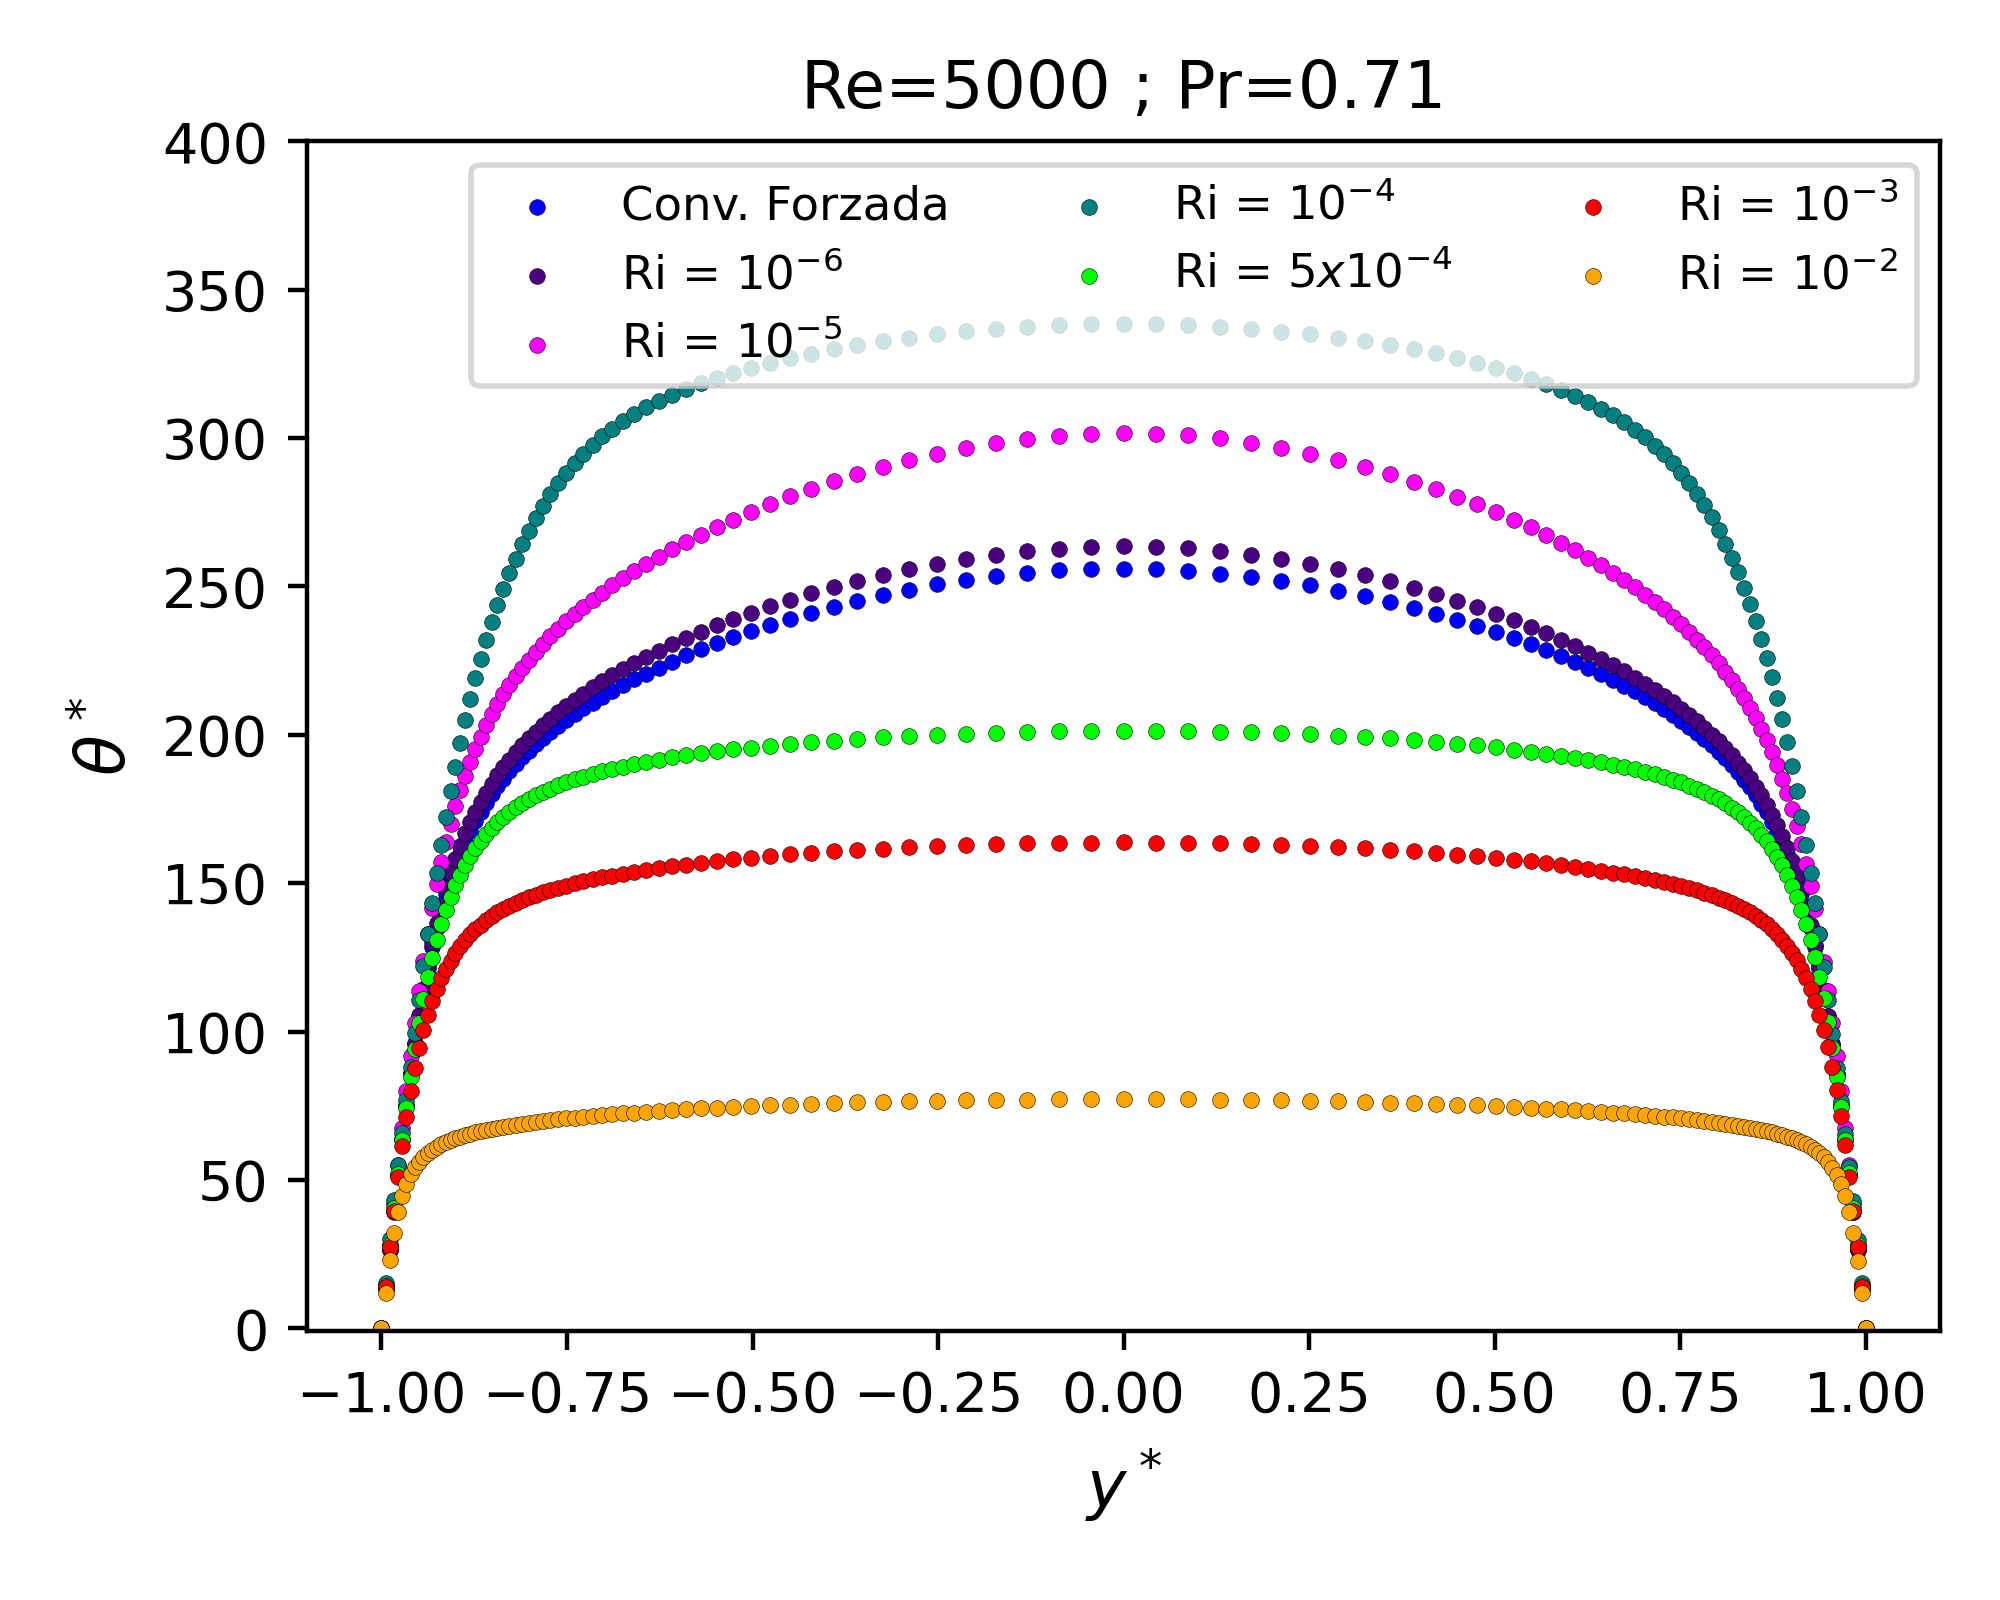
\includegraphics[width=0.49\textwidth]{figures/cap5/Re5000-Pr071/phi_mean_profile.png}
    	\label{fig:phi-Re5000-Pr071}}
  \caption{Perfiles medios adimensionales de \textbf{(a)} velocidad y \textbf{(b)} temperatura, para varios Ri$_b$.}
\end{figure}

Por otra parte, la Figura \ref{fig:phi-Re5000-Pr071} presenta los perfiles medios de temperatura adimensional. A diferencia de los perfiles de velocidad, estos no exhiben la configuración en ``M'' pero sí un comportamiento no monótono con el incremento del Ri$_b$ \cite{you2003direct, steiner1971reverse}. Los casos pueden clasificarse, en primera instancia, en dos conjuntos:

\begin{itemize}

\item[\textbf{(I)}] valores de Ri$_b$ comprendidos entre 0.04 y 1.06;

\item[\textbf{(II)}] valores de Ri$_b$ entre 5.33 y 106.5.

\end{itemize}
Los mismos exhiben comportamientos físicos claramente diferenciados. Esta distinción se analizará en detalle a lo largo de la presente sección.

En el primer conjunto se aprecia un aumento del perfil adimensional respecto al caso de convección forzada, lo que equivale a decir que aunque se aumente el flujo de calor, la diferencia de temperaturas entre el centro del canal y la pared se incrementa, sugiriendo una disminución de la eficiencia en la transferencia de calor. Cuando la fuerza boyante se intensifica aún más (conjunto \textbf{II}) este efecto se revierte y la temperatura adimensional disminuye, lo que indica que un aumento del Ri$_b$ produce una menor diferencia entre la temperatura en el centro del canal y la temperatura en la pared. Asimismo, en este segundo conjunto, los perfiles presentan una forma más ``achatada'' en el seno del canal respecto al primer conjunto. Esto puede interpretarse cualitativamente a partir de los perfiles de velocidad: una mayor diferencia de velocidades entre la región próxima a la pared y el centro del canal favorece la mezcla del fluido y, por consiguiente, conduce a una distribución térmica más homogénea \cite{aicher1997}.

\newpage
\subsection{Valores RMS de temperatura y velocidad} 

Las Figuras \ref{fig:rms-ux-Re5000-Pr071} y \ref{fig:rms-phi-Re5000-Pr071} muestran los perfiles de las fluctuaciones de velocidad \textit{streamwise} y temperatura adimensional, respectivamente. Partiendo del caso puramente forzado, el incremento de la fuerza boyante provoca evoluciones distintas en los conjuntos \textbf{I} y \textbf{II} considerados anteriormente. En el primero, se observa una disminución (incremento) de las fluctuaciones de velocidad (temperatura) seguida de una ligera recuperación (leve descenso). En el segundo, las fluctuaciones de velocidad crecen de manera sostenida a medida que la fuerza boyante se intensifica, mientras que las de temperatura tienden a reducirse. Tendencias análogas han sido descritas por otros autores \cite{you2003direct,carr1973velocity}.

\begin{figure}[H]
  \centering
  
  \subfloat[]{
    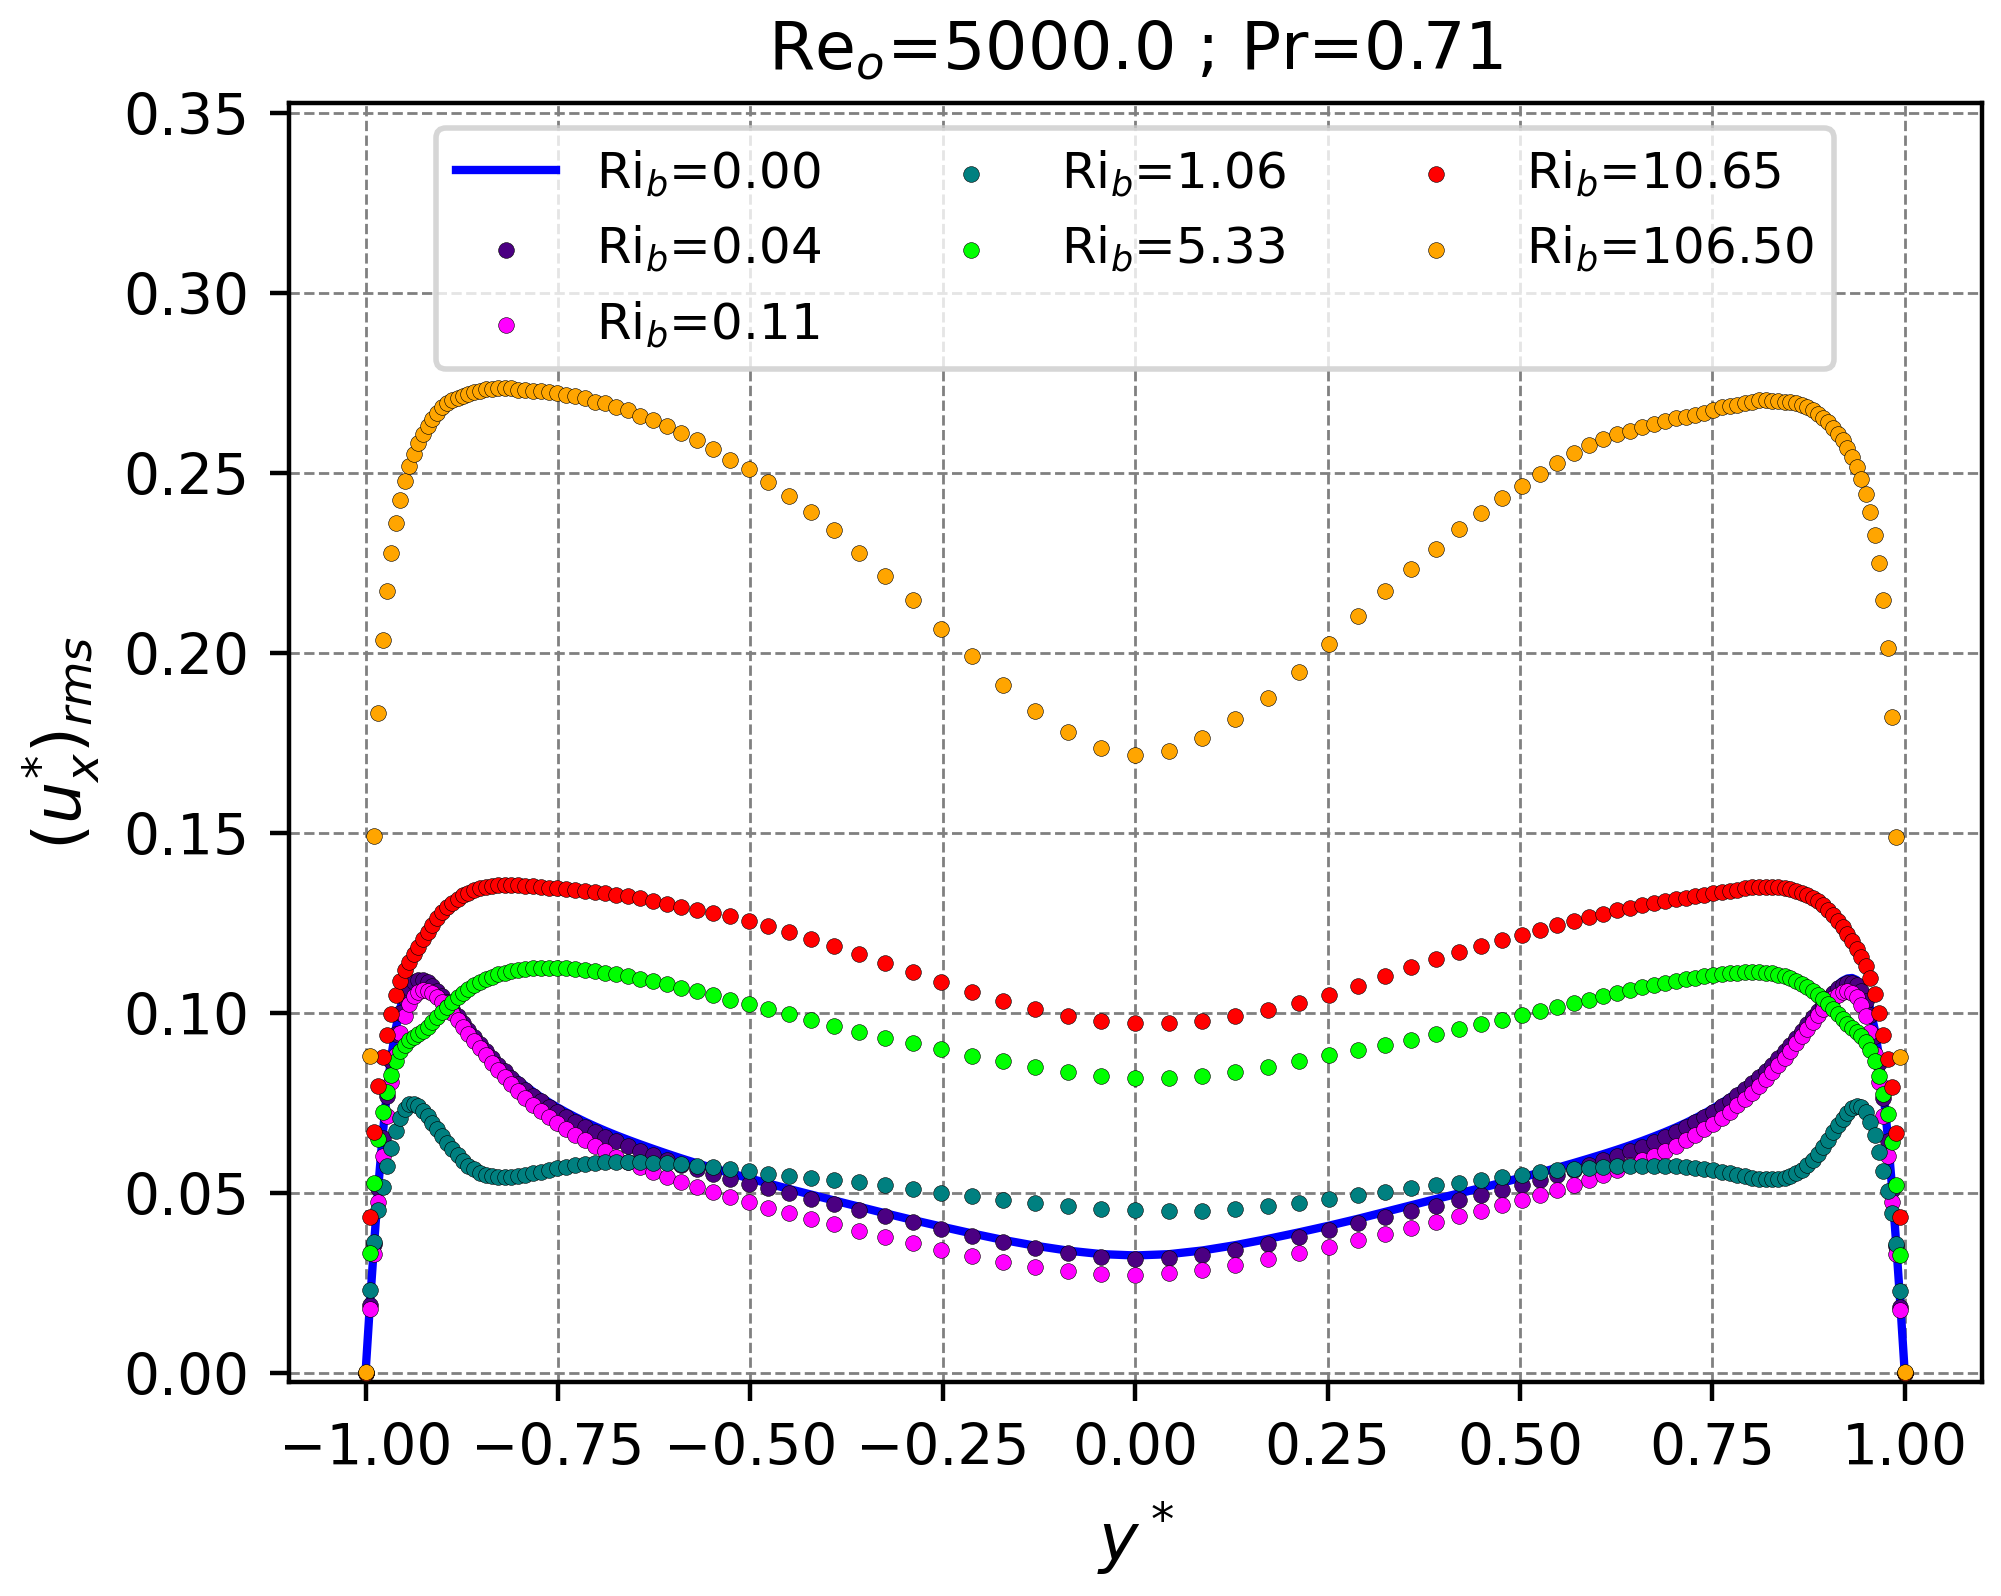
\includegraphics[width=0.49\textwidth]{figures/cap5/Re5000-Pr071/ux_rms_profile.png}
     \label{fig:rms-ux-Re5000-Pr071}}
  \subfloat[]{
    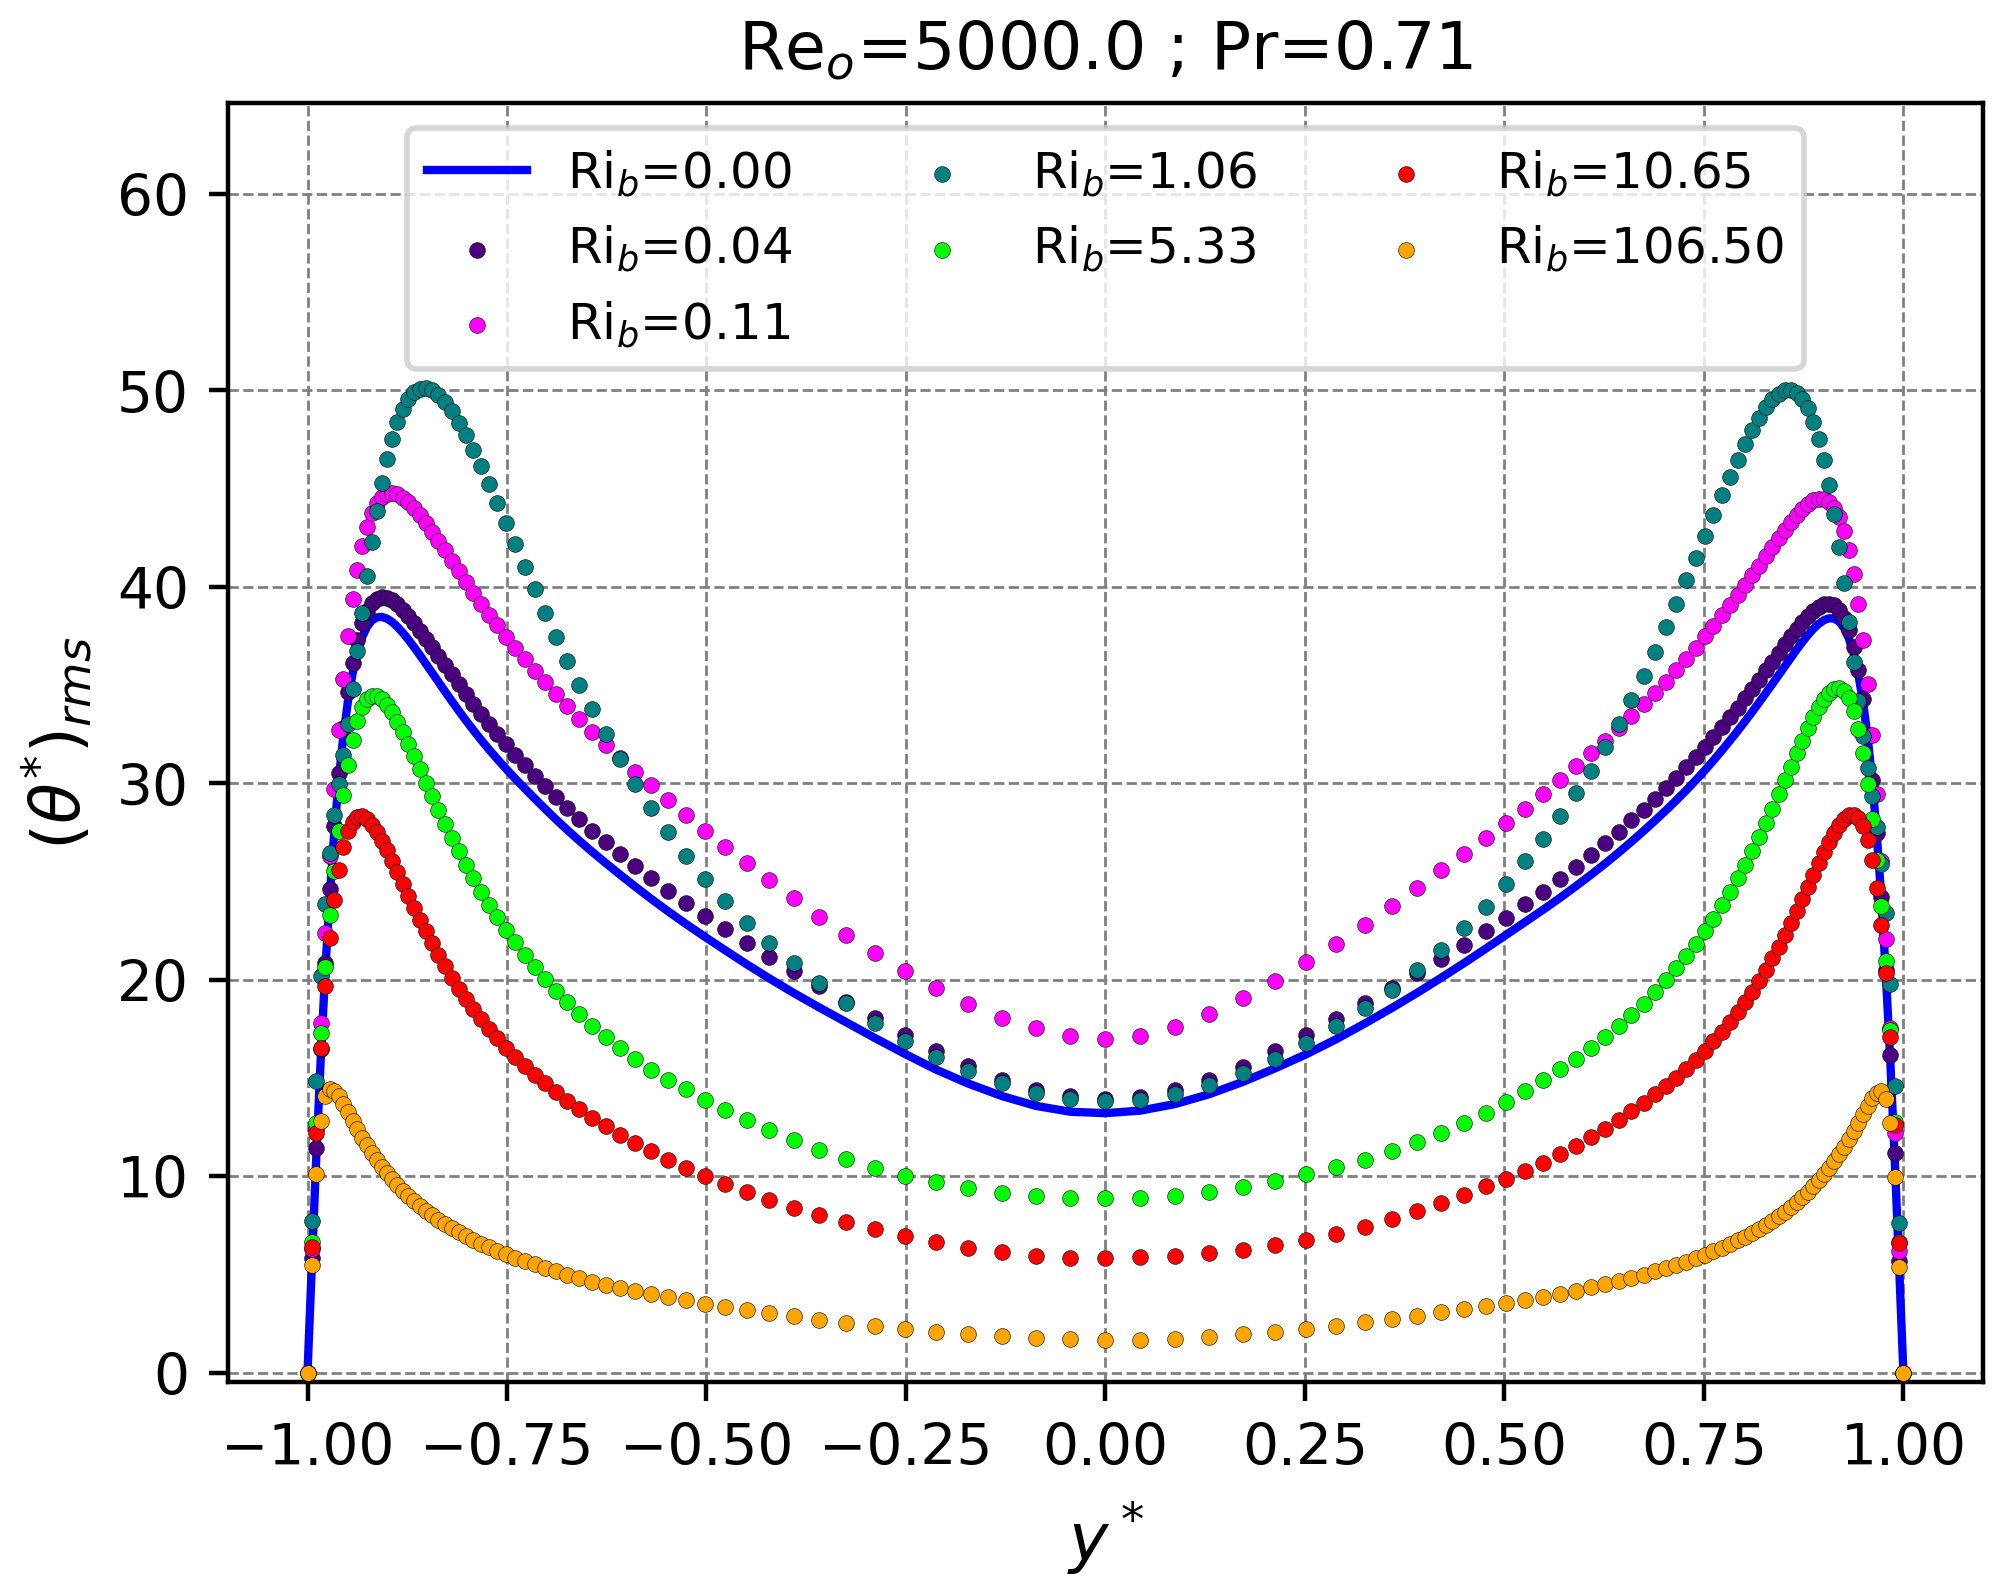
\includegraphics[width=0.49\textwidth]{figures/cap5/Re5000-Pr071/phi_rms_profile.png}
    \label{fig:rms-phi-Re5000-Pr071}}
    \caption{Fluctuaciones RMS: \textbf{(a)} velocidad en la dirección de la corriente y \textbf{(b)} temperatura adimensional.}
    \label{fig:rms-Re5000-Pr071}
\end{figure}

Como se aprecia en la Figura \ref{fig:rms-ux-Re5000-Pr071}, la aparición de la fuerza boyante de baja intensidad relativa, por ejemplo, en el caso con $\text{Ri}_b=1\text{.}06$, produce primero una leve estabilización del flujo, evidenciada por una disminución de aproximadamente un 40$\%$ en los máximos de $(u^*_x)_{rms}$ próximos a las paredes. En contraste, las fluctuaciones de temperatura adimensional aumentan y sus máximos se desplazan hacia el centro del canal debido al incremento del flujo de calor. Para $\text{Ri}_b=5\text{.}33$ la fuerza boyante adquiere mayor preponderancia y las fluctuaciones de velocidad crecen en todo el ancho del canal; por ejemplo, en el caso de $\text{Ri}_b=10\text{.}65$ el valor en el centro es aproximadamente un 70$\%$ mayor respecto al caso con $\text{Ri}_b=1\text{.}06$. Este incremento de la agitación dinámica redistribuye las fluctuaciones de temperatura, que disminuyen en magnitud respecto al caso de convección forzada (Figura \ref{fig:rms-phi-Re5000-Pr071}).

\subsection{Flujos turbulentos de calor} 

En la Figura \ref{fig:uxphi_f-Re5000-Pr071} se expone el perfil de la correlación $\langle u_x^{\ast \prime } \theta^{\ast \prime } \rangle$. Esta cantidad corresponde al flujo de calor turbulento \textit{streamwise} que surge a raíz del desarrollo de la ecuación de conservación de energía promediada (véase Apéndice \ref{apen:budgets}), y puede interpretarse como el calor transportado por las estructuras producidas por el flujo turbulento.  

\begin{figure}[H]
  \centering
  \subfloat[]{
    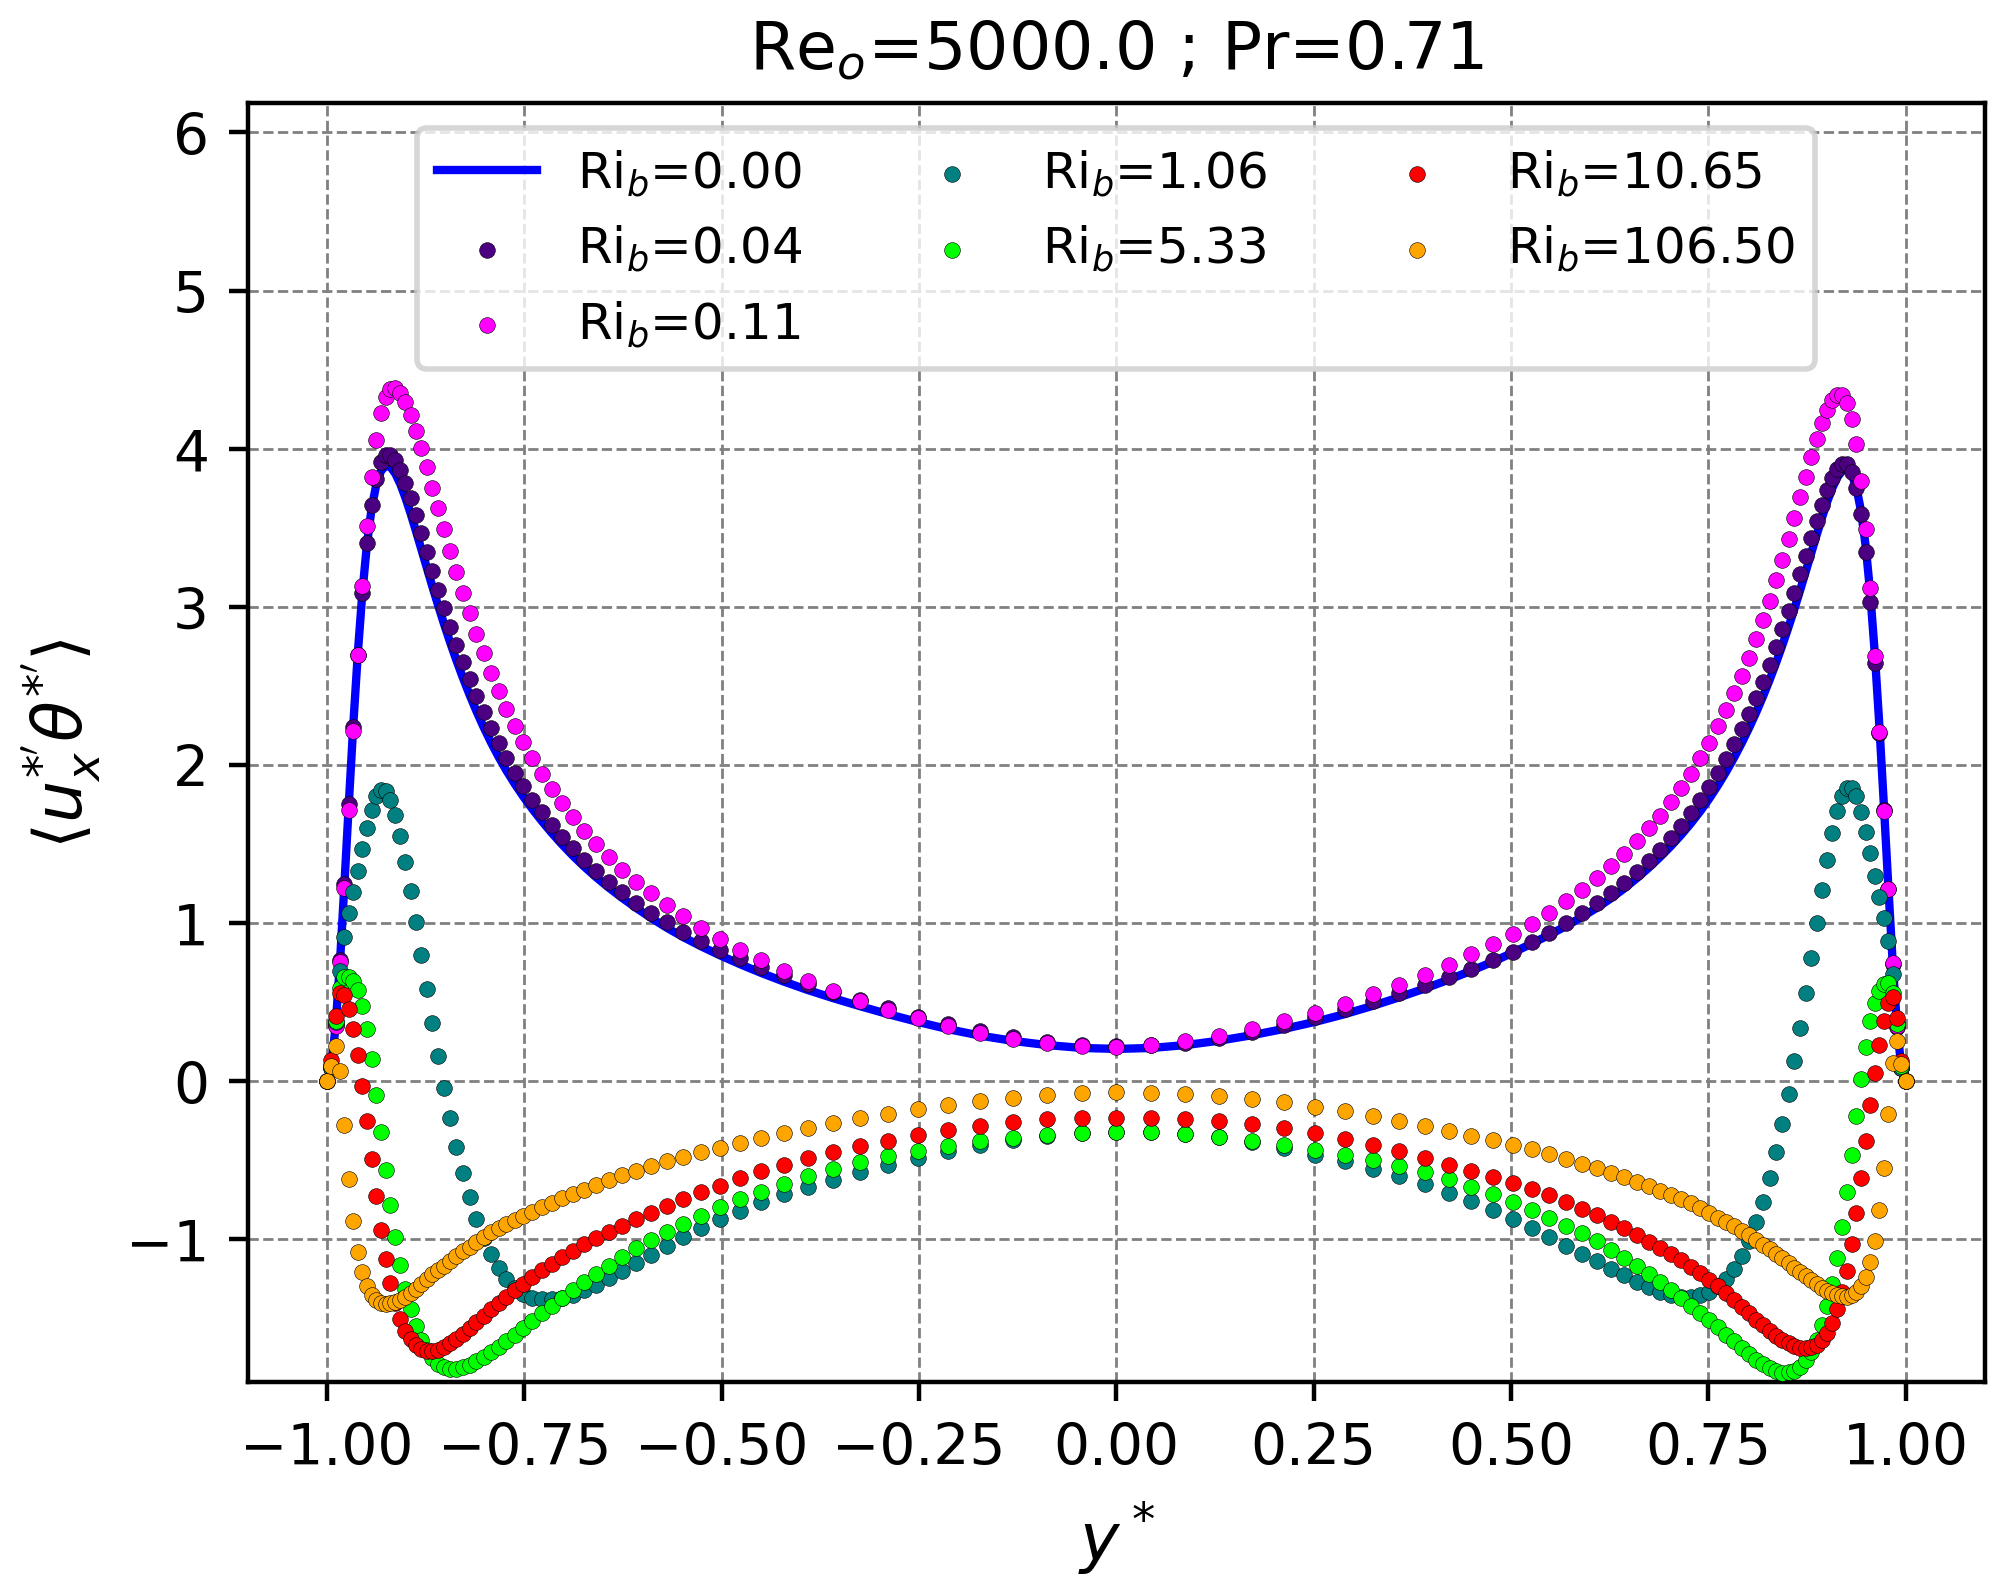
\includegraphics[width=0.53\textwidth]{figures/cap5/Re5000-Pr071/uxphif_profile.png}
    \label{fig:uxphi_f-Re5000-Pr071}}
  \subfloat[]{
    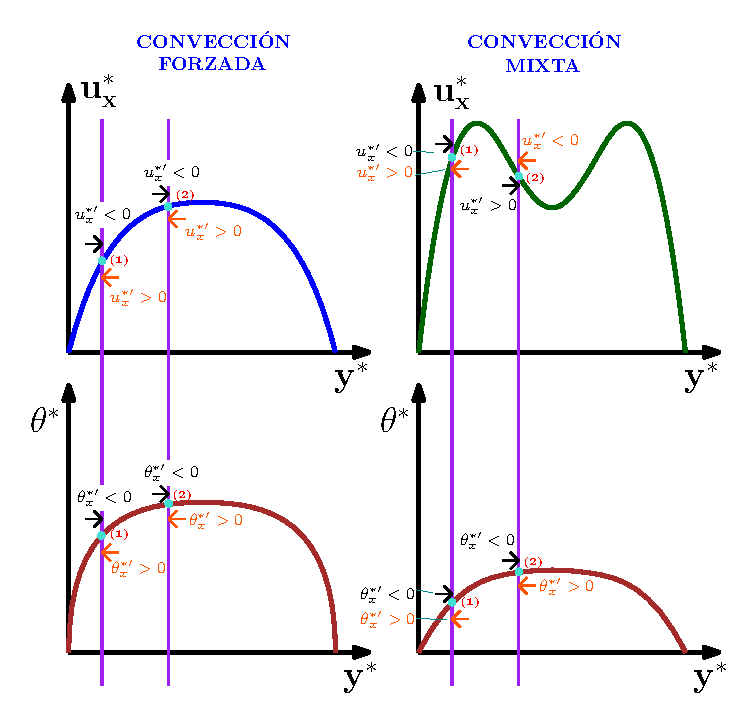
\includegraphics[width=0.46\textwidth]{figures/cap5/Re5000-Pr071/uxphif_esquema.eps}
     \label{fig:uxphi_esquema-Re5000-Pr071}}
    \caption{\textbf{(a)} Flujo de calor turbulento en la dirección de la corriente. \textbf{(b)} Esquema de perfiles de temperatura y velocidad para convección forzada y mixta. Aquí los desplazamientos $dy^*$ hacia la izquierda (derecha) están representados con flechas anaranjadas (negras).}
    \label{fig:rms-Re5000-Pr071}
\end{figure}

En el seno del canal se aprecia una diferencia marcada (signo del flujo de calor turbulento) entre el caso forzado y aquellos con fuerza boyante relativamente débil (Ri$_b$=0.04, 0.11; signo positivo), respecto al resto de casos (signo negativo). Esta disparidad se puede entender cualitativamente a través de los perfiles de $u^*_x$ y $\theta^*$. Para ello, en la Figura \ref{fig:uxphi_esquema-Re5000-Pr071} se muestran los perfiles esquemáticos de ambas magnitudes para los regímenes de convección forzada y mixta:

\begin{itemize}

\item \textbf{Cerca de la pared.} Analizando el caso forzado, supóngase que una partícula de fluido próxima a la pared se desplaza un diferencial $dy^*$ a la derecha debido a una fluctuación ($u^{* \prime}_y >0$) y arriba al \textbf{Punto (1)}. Entonces, en dicho punto, se produce una fluctuación negativa en la velocidad \textit{streamwise} ($u^{* \prime}_x <0$) y la partícula se traslada de una zona más fría a una más caliente, y por lo tanto, experimenta una fluctuación negativa en su temperatura adimensional ($\theta^{* \prime}<0$). Esto se traduce en una correlación positiva $\langle u_x^{\ast \prime } \theta^{\ast \prime } \rangle > 0$. 

Por otro lado, si la partícula de fluido llega al \textbf{Punto (1)} al desplazarse un diferencial $dy^*$ a la izquierda ($u^{* \prime}_y <0$), se genera una fluctuación positiva en la velocidad \textit{streamwise}  ($u^{* \prime}_x >0$) y la misma se desplaza de una región caliente a una más fría. En consecuencia, $\theta^{* \prime}$ es positiva y se produce nuevamente una correlación positiva.

La situación es completamente análoga para el caso de convección mixta.

\item \textbf{Cerca del centro del canal.} En el caso de convección forzada la situación es idéntica a la encontrada cerca de la pared. Por lo cual, en el caso forzado se tiene una correlación positiva global que es consistente con lo que se observa en la Figura \ref{fig:uxphi_f-Re5000-Pr071}. 

Sin embargo, si uno realiza el mismo análisis para el caso de convección mixta, ocurre lo contrario. En otras palabras, debido a una fluctuación $u^{* \prime}_y >0$ ($u^{* \prime}_y <0$) ocurre un desplazamiento $dy^*$ a la derecha (izquierda), la partícula arriba al \textbf{Punto (2)}. Entonces, se produce una fluctuación positiva (negativa) de la velocidad \textit{streamwise}  y la partícula se traslada de una región más fría (caliente) a una más caliente (fría). Esto da como resultado una fluctuación negativa de la temperatura adimensional en ambas situaciones y por lo tanto, en el seno del canal, la correlación $\langle u_x^{\ast \prime } \theta^{\ast \prime } \rangle$ es negativa en consonancia con lo observado en los perfiles.
\end{itemize}  
Del análisis anterior, puede afirmarse que la disparidad entre los conjuntos \textbf{I} y \textbf{II} en la magnitud analizada se debe al cambio de concavidad del perfil de velocidad en el seno del canal. Esto último es inducido por el aumento de la fuerza boyante. 

Adicionalmente, es importante mencionar que esta cantidad, el flujo de calor turbulento \textit{streamwise}, actúa como un término de producción en la ecuación de la energía cinética turbulenta y contribuye a su aumento cuando es negativo (véase Apéndice \ref{apen:budgets}).


\begin{figure}[H] % usa [H] solo si necesitas anclarla y tienes \usepackage{float}
  \centering
  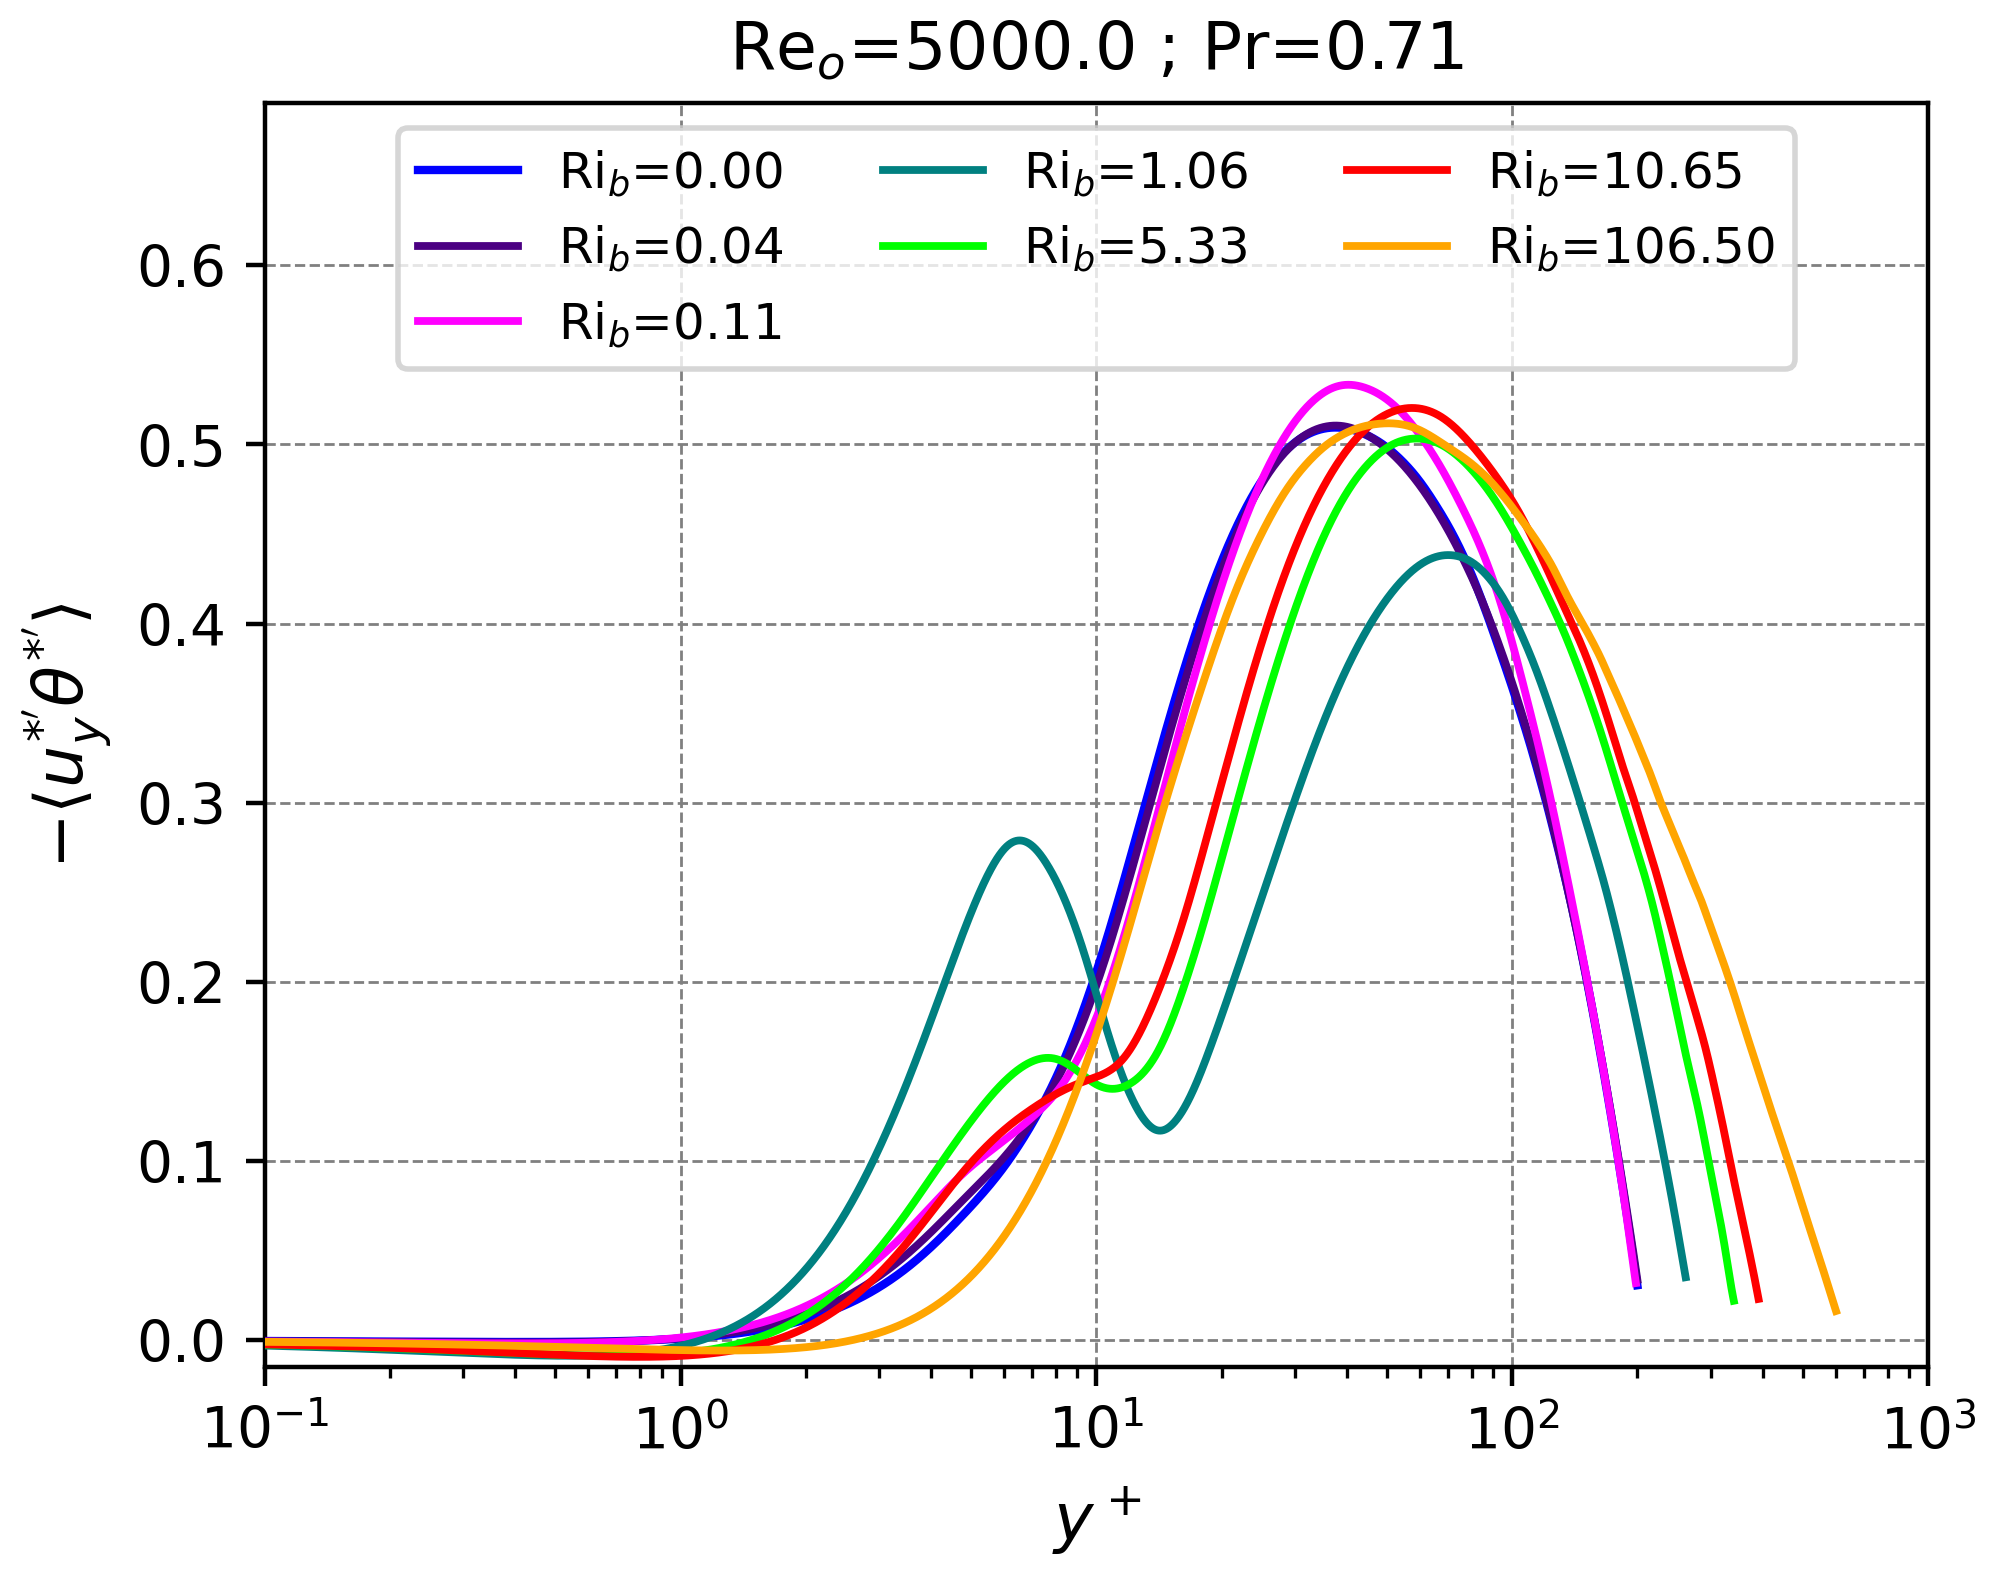
\includegraphics[width=0.5\textwidth]{figures/cap5/Re5000-Pr071/uyphif_profile.png}  
  \caption{Perfil del flujo de calor turbulento en la dirección normal a la pared donde la abscisa se encuentra expresada en unidades de pared (\textit{wall units}).}
  \label{fig:uyphi_f-Re5000-Pr071}
\end{figure}

Por último, en la Figura \ref{fig:uyphi_f-Re5000-Pr071} se expone el perfil del flujo de calor turbulento en la dirección normal a la pared: $-\langle u_y^{\ast \prime } \theta^{\ast \prime } \rangle$. Nótese que la abscisa de este gráfico se encuentra en unidades de pared para visualizar claramente el comportamiento cercano a la misma.   Considerando nuevamente el conjunto \textbf{I} (Ri$_b$=0.04, 0.11, 1.06), se observa que los máximos tienden a desplazarse levemente hacia el seno del canal. Un comportamiento similar se observa en \cite{you2003direct}. Por otro lado, en el conjunto \textbf{II}, los máximos tienden a desplazarse hacia la pared. Asimismo, muy próximo a la pared, para los casos con Ri$_b$=0, 0.04, 0.11, 10.65, 106.5 el perfil se comporta de forma monótona creciente, mientras que en el resto de casos (Ri$_b$=1.06, 5.33) se observa un máximo y mínimo local. Se especula que estos máximos y mínimos locales, que están dentro y cerca del límite de la capa conductiva, están asociados a la distancia a la cual ocurren los picos de $\langle u_y^{\ast \prime } u_y^{\ast \prime } \rangle$ y $\langle \theta^{\ast \prime } \theta^{\ast \prime } \rangle$, es decir, a las intensidades de las fluctuaciones de las dos variables involucradas.



\section{Comparación entre casos de distinto Prandtl}

En esta sección se comparan los casos con los siguientes parámetros: Re$_o$=5000; Pr=0.071, 0.71; Ri$_b$=0.11, 1.06, 10.65. La Figura \ref{fig:ux-plus-Re5000-Pr071} muestra los perfiles de velocidad media expresados en unidades de pared (\textit{wall units}). Según Pope \cite{pope2001turbulent}, en la subcapa viscosa ($y^+ < 5$), la velocidad puede aproximarse por
$$\langle u_x^+ \rangle \;\simeq\; y^+ + \mathcal{O} \left[(y^+)^{2} \right]\text{ .}$$
Esta ley, conocida como ley de pared (\textit{Wall-Law}), se indica en la Figura \ref{fig:ux-wall-law-Re5000-Pr071} con la línea negra de referencia. En dicha región las tensiones de Reynolds son despreciables frente a las tensiones viscosas, de modo que el perfil depende casi exclusivamente de la distancia normalizada a la pared. Como puede verse, todos los casos, independientemente del número de Prandtl y de la fuerza boyante, siguen de cerca esta aproximación lineal, lo que confirma la validez de la ley en la subcapa viscosa. 

Por otra parte, en la región logarítmica (\textit{log-law region}), en condiciones de convección forzada, la velocidad media en la dirección de la corriente se alinea perfectamente con la ley logarítmica clásica \cite{kawamura2000dns} como se observa en la Figura \ref{fig:ux-log-law-Re5000-Pr071}. Nótese, además, que el caso con Pr=0.71 y Ri$_b$=0.11 (fuerza boyante de baja intensidad relativa), se encuentra también en buen acuerdo con la ley logarítmica. Sin embargo, esta ley deja de ser aplicable cuando la flotabilidad es significativa \cite{zhou2024direct}.

\begin{figure}[H]
  \centering
  \subfloat[]{
    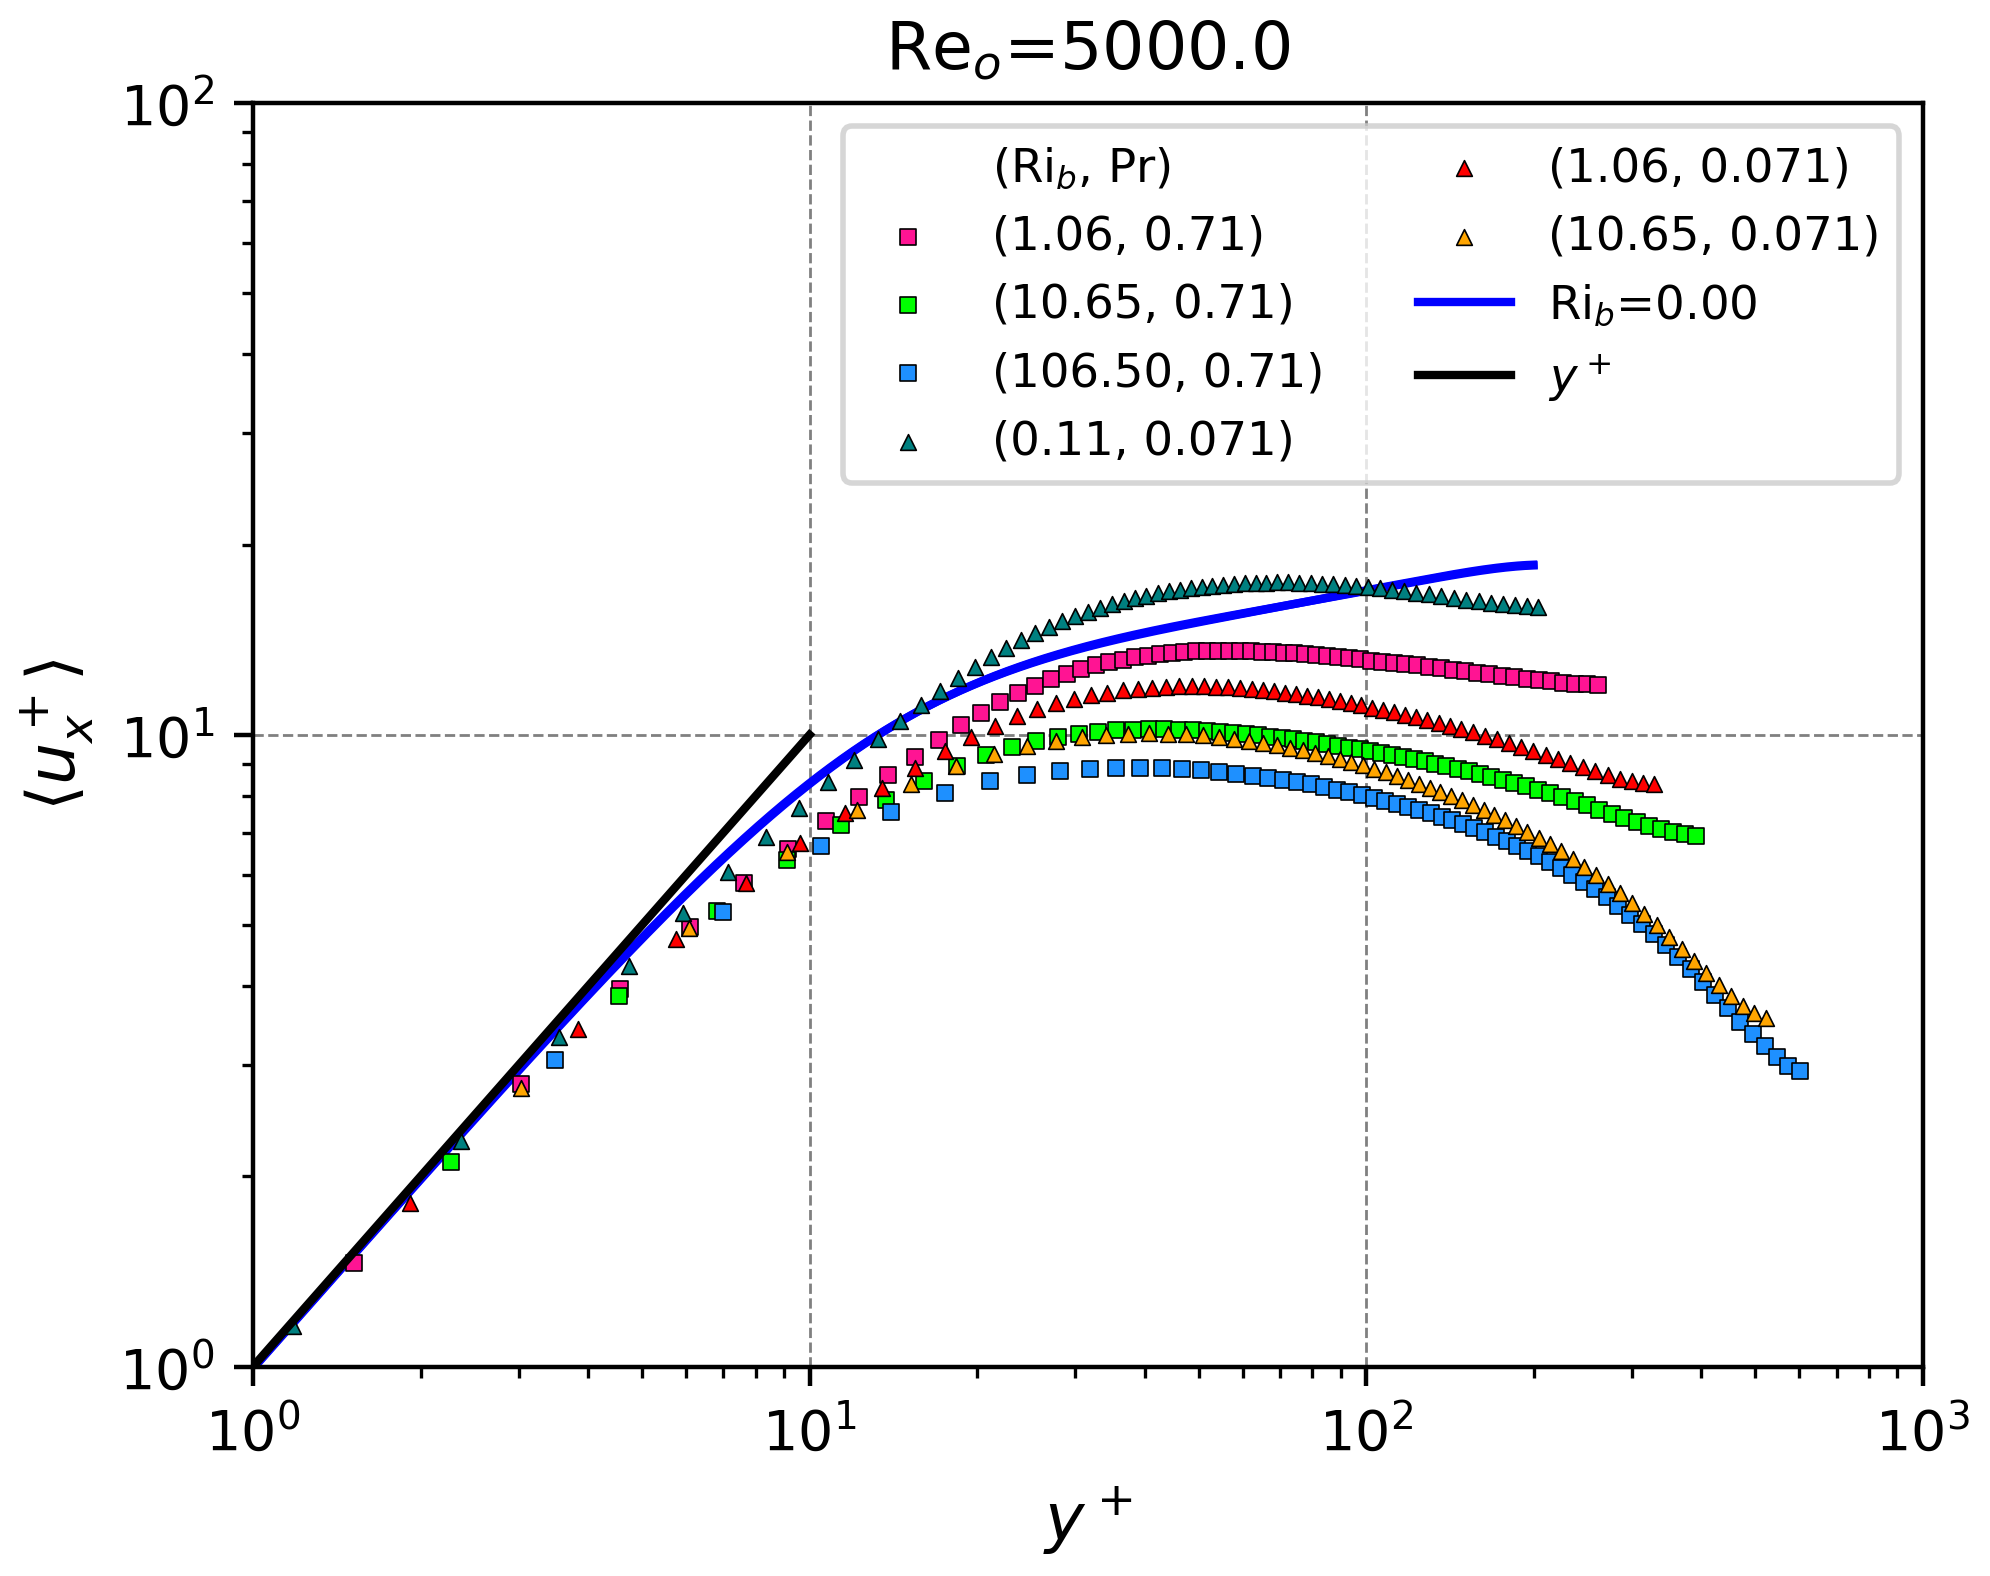
\includegraphics[width=0.49\textwidth]{figures/cap5/Re5000-Pr071/ux_mean_plus_log_profile_wall_law.png}
    \label{fig:ux-wall-law-Re5000-Pr071}}
  \subfloat[]{
    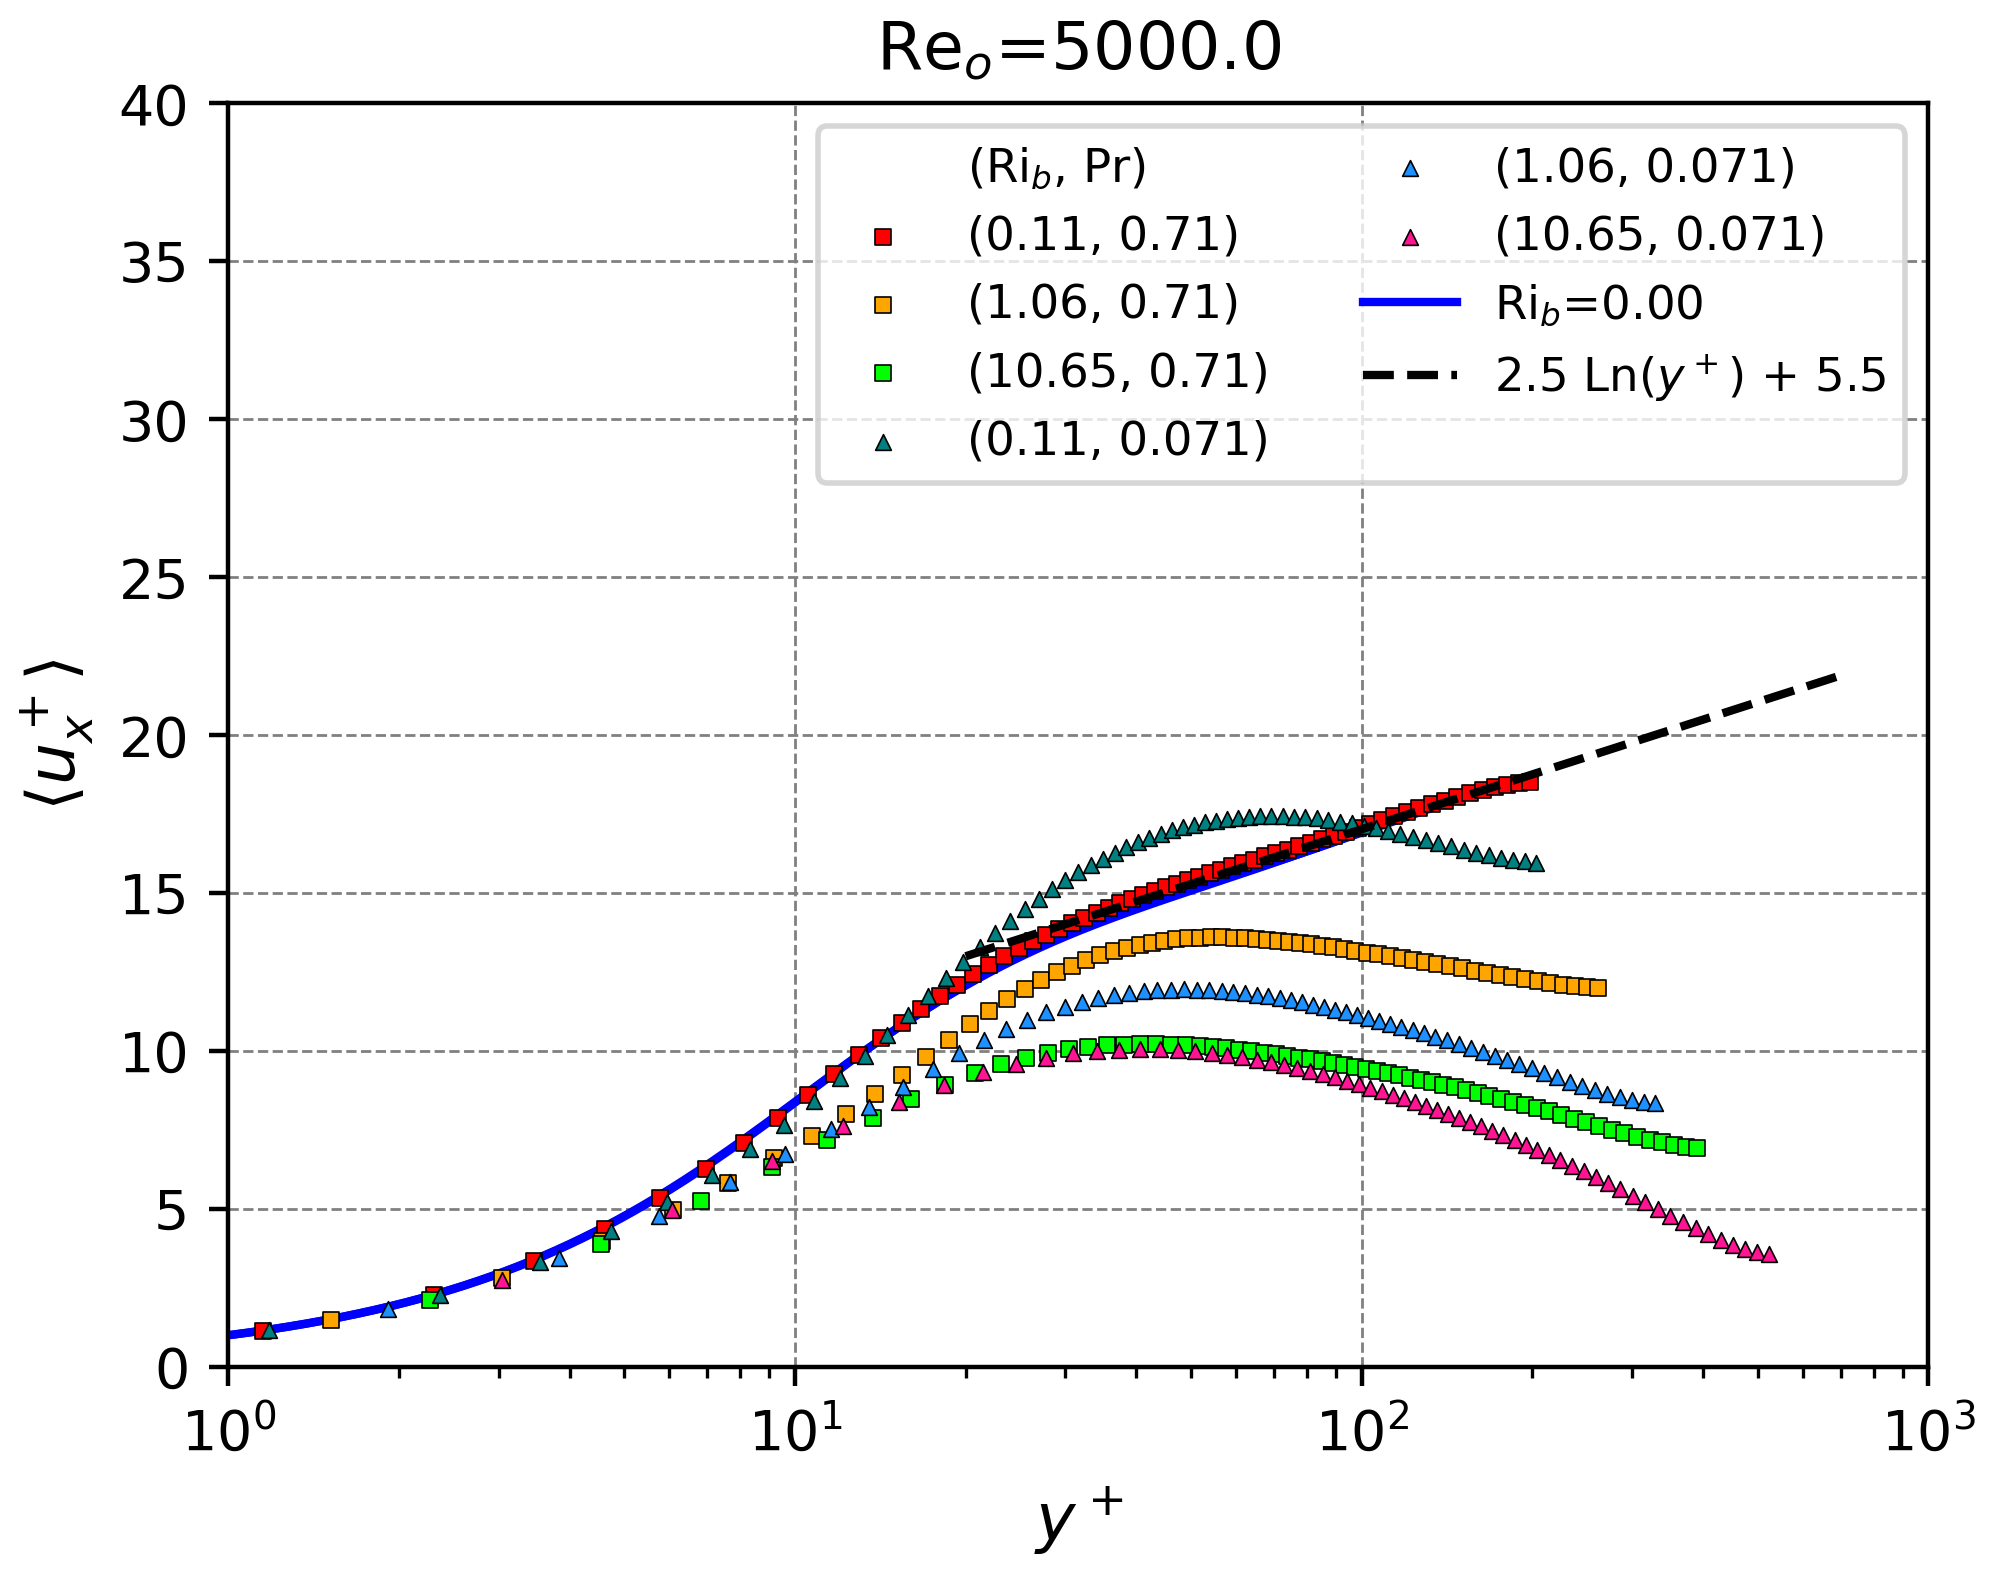
\includegraphics[width=0.49\textwidth]{figures/cap5/Re5000-Pr071/ux_mean_plus_log_profile_log_law.png}
     \label{fig:ux-log-law-Re5000-Pr071}}
    \caption{Perfiles medios de velocidad en unidades de pared para Re$_o$=5000 y Pr=0.071, 0.71, y distintos valores de Ri$_b$. \textbf{(a)} \textit{Wall-Law}. \textbf{(b)} \textit{Log-Law}. }
    \label{fig:ux-plus-Re5000-Pr071}
\end{figure}

La Figura \ref{fig:phi-plus-Re5000-Pr071} muestra los perfiles de temperatura adimensional media en unidades de pared. Cerca de la pared, la variación de la temperatura puede aproximarse por la relación lineal \cite{kawamura1998dns}
\begin{equation*}
\langle \theta^* \rangle \simeq \text{Pr}\hspace{0.5mm} y^+ ,
\end{equation*}
representada en la Figura \ref{fig:phi-wall-law-Re5000-Pr071} con líneas negras. Los resultados confirman esta ley para ambos números de Prandtl, aunque con distintos alcances: para el caso de Pr=0.071 la validez se extiende hasta $y^{+}\approx 30$, en concordancia con el trabajo de Zhou et al. \cite{zhou2024direct}. Sin embargo, para Pr=0.71 se reduce a $y^{+}\approx 7$. La diferencia recae en que, en fluidos con mayor difusividad térmica (Prandtl más bajo), el transporte de calor por conducción domina durante una mayor distancia normalizada desde la pared, retrasando la aparición del régimen convectivo predominante \cite{abregu2023dns}.

\begin{figure}[H]
  \centering
  \subfloat[]{
    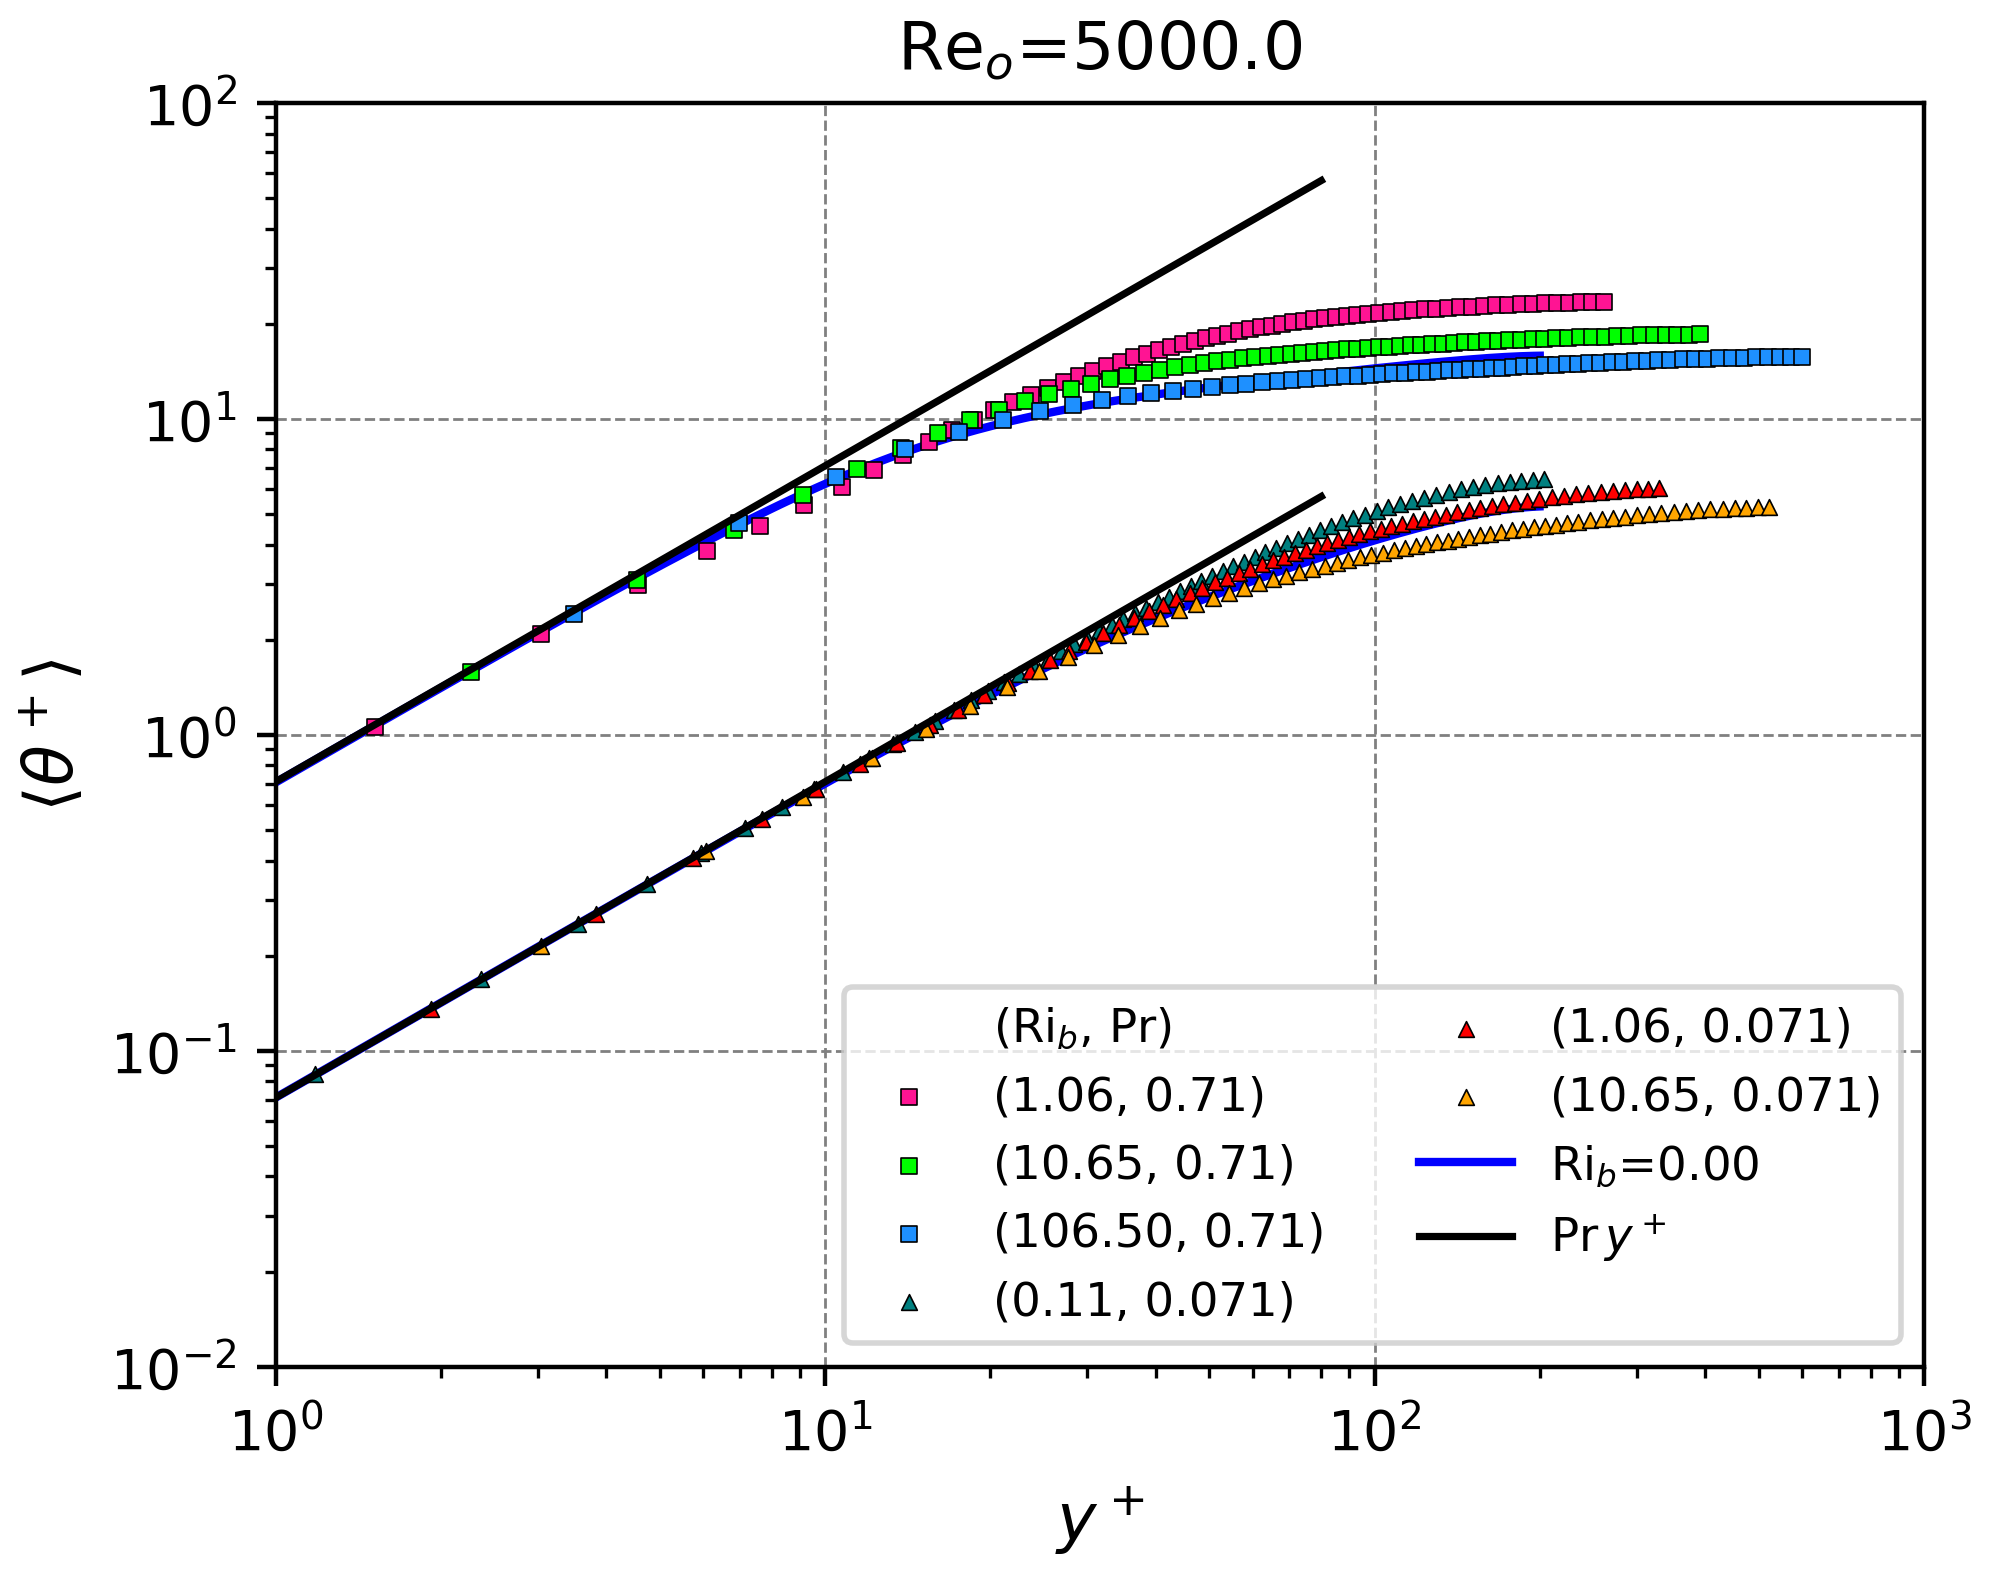
\includegraphics[width=0.49\textwidth]{figures/cap5/Re5000-Pr071/phi_mean_plus_log_profile_wall_law.png}
    \label{fig:phi-wall-law-Re5000-Pr071}}
  \subfloat[]{
    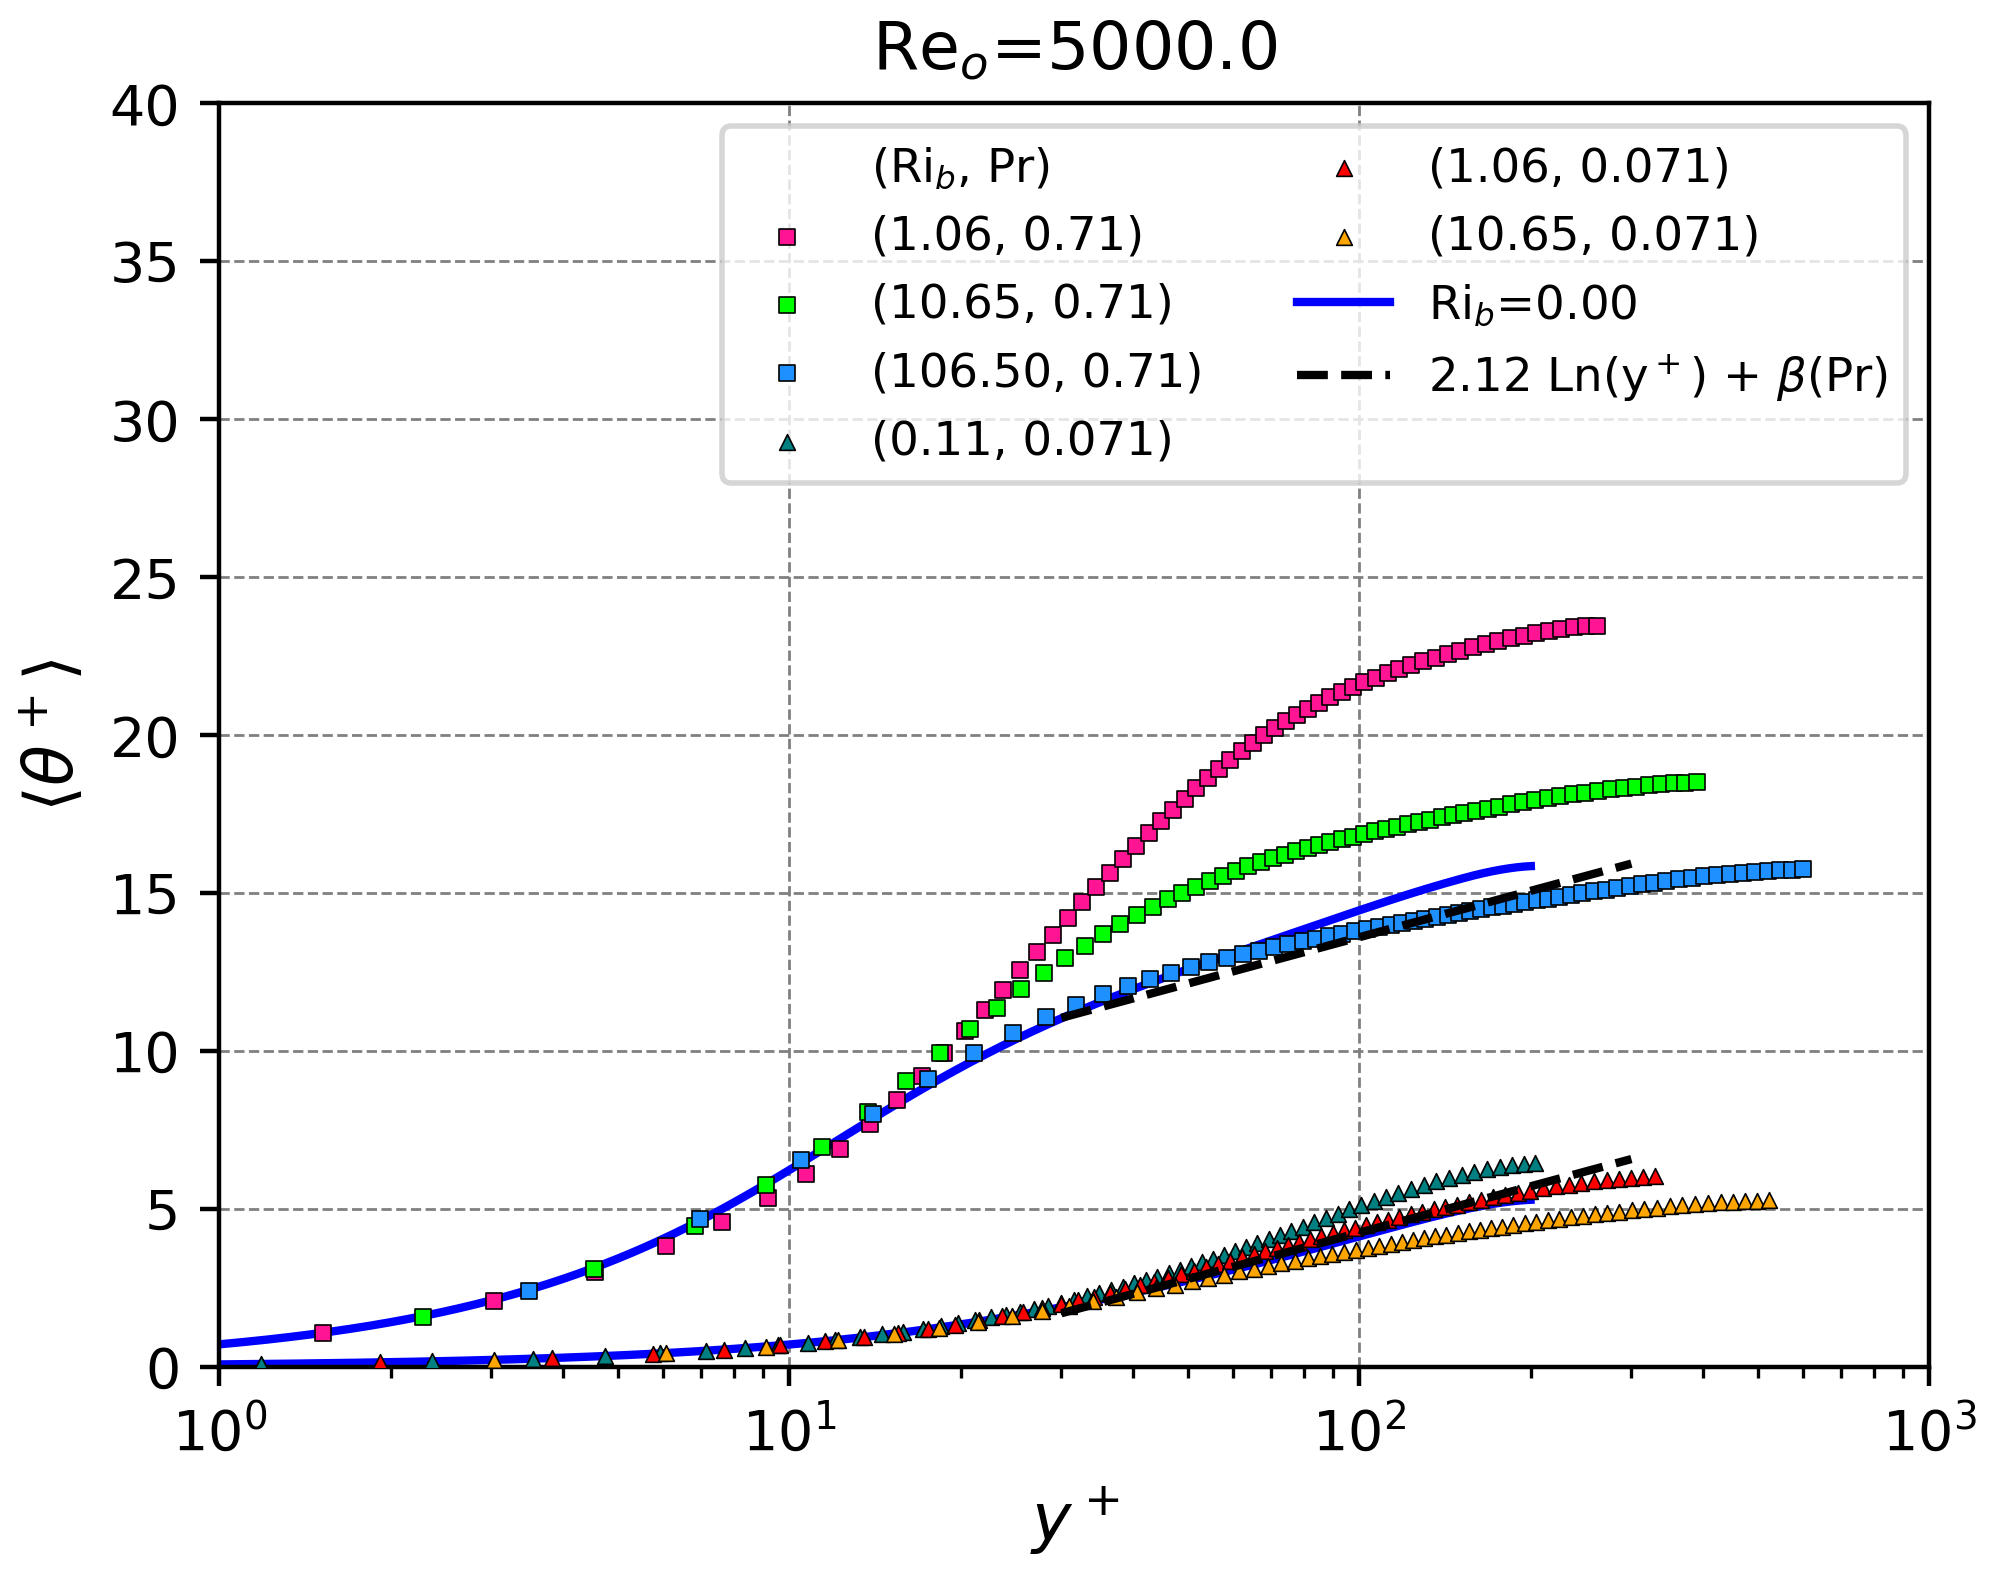
\includegraphics[width=0.49\textwidth]{figures/cap5/Re5000-Pr071/phi_mean_plus_log_profile_log_law.png}
     \label{fig:phi-log-law-Re5000-Pr071}}
    \caption{Perfiles medios de temperatura en unidades de pared para Re$_o$=5000 y Pr=0.071, 0.71, y distintos valores de Ri$_b$. \textbf{(a)} \textit{Wall-Law}. \textbf{(b)} \textit{Log-Law}.}
    \label{fig:phi-plus-Re5000-Pr071}
\end{figure}

%En la región logarítmica, la ley de pared para temperatura propuesta por Kader \cite{kader1981temperature} puede escribirse, de manera genérica, como
%
%\begin{equation*}
%\langle \theta^* \rangle \simeq A \ln(y^+) + \beta(\text{Pr}) \text{,}
%\end{equation*}
%donde $\beta$ es la constante aditiva (dependiente de Pr). En la Figura \ref{fig:phi-log-law-Re5000-Pr071} (línea a trazos negra). se observa que, para $\text{Pr}=0\text{.}071$ ($\beta=-5\text{.}52$), hay un buen acuerdo tanto para el caso de convección forzada como para el correspondiente a $\text{Ri}_b=1\text{.}06$, con validez en el rango $30<y^+<200$. En cambio, para $\text{Pr}=0\text{.}71$, la formulación de Kader ($\beta=3\text{.}83$) presenta discrepancias tanto en convección forzada como en los casos de convección mixta.
%
%Adicionalmente, se incluye la ley logarítmica de Kasagi et al. \cite{kasagi1992direct} (línea a trazos verde en la Figura \ref{fig:phi-log-law-Re5000-Pr071}) que reproduce con mayor fidelidad el comportamiento del caso de convección forzada. En términos generales, puede apreciarse visualmente que, para cierto intervalo $a_{\text{min}}<y^+<a_{\text{max}}$ con $y^+>30$ y $a_{\text{min}},a_{\text{max}}\in[30,300]$, cada caso (considerado de manera individual) admite una descripción tipo logarítmica en ese subrango cuya pendiente y ordenada al origen se determinan ajustando los datos. Este aspecto se documenta aquí como observación y se considera materia de trabajo futuro.

En la región logarítmica, la ley de pared para la temperatura propuesta por Kader \cite{kader1981temperature} puede escribirse, de manera genérica, como
\begin{equation*}
\langle \theta^* \rangle \simeq A \ln(y^+) + \beta(\text{Pr}),
\end{equation*}
donde $A$ es la pendiente ($A \simeq 2\text{.}12$) y $\beta$ es una constante aditiva (dependiente de $\text{Pr}$). En la Figura \ref{fig:phi-log-law-Re5000-Pr071} (línea a trazos negra) se observa que, para $\text{Pr}=0\text{.}071$ ($\beta=-5\text{.}52$), hay un buen acuerdo tanto para el caso de convección forzada como para el correspondiente a $\text{Ri}_b=1\text{.}06$, con validez en el rango $30<y^+<200$. En cambio, para $\text{Pr}=0\text{.}71$, la formulación de Kader ($\beta=3\text{.}83$) presenta discrepancias tanto en convección forzada como en los casos de convección mixta.

Adicionalmente, se incluye la ley logarítmica de Kasagi et al. \cite{kasagi1992direct} (línea a trazos verde en la Figura \ref{fig:phi-log-law-Re5000-Pr071}), que reproduce con mayor fidelidad el comportamiento del caso de convección forzada. En términos generales, puede apreciarse visualmente que, para cierto intervalo $a_{\text{min}}<y^+<a_{\text{max}}$ con $y^+>30$ y $a_{\text{min}},a_{\text{max}}\in[30,300]$, cada caso (considerado de manera individual) admite una descripción de tipo logarítmico en ese subrango, con pendiente y ordenada al origen determinadas mediante ajuste de los datos. Este aspecto se documenta aquí como observación y se considera materia de trabajo futuro.



\newpage
\section{Número de Nusselt} \label{sec:nu}

Desde una perspectiva ingenieril, el número de Nusselt (Nu) es un indicador clave de la eficiencia de la transferencia de calor. Su definición se presenta en la ecuación \ref{eq:nu}, donde $\langle \theta_b \rangle$ es la temperatura \textit{bulk} (ecuación \ref{eq:tita_bulk}).

\begin{align}
&\text{Nu} = \frac{h L}{k} = \frac{2d}{k} \frac{q''_w}{\langle \theta_b \rangle} = \frac{4}{3} \frac{Re_o Pr}{\langle \theta^*_b \rangle}	
\label{eq:nu} \\
&\langle \theta_b \rangle = \frac{\int_{-d}^{+d} \langle u_x \theta \rangle \, dy}{\int_{-d}^{+d} \langle u_x \rangle \, dy} = \frac{\int_{-d}^{+d} \langle u_x \theta \rangle }{2d \, U_b}
\label{eq:tita_bulk}
\end{align}

La Figura \ref{fig:nu_vs_bo} muestra los valores de Nu obtenidos en función del número de boyancia Bo (ecuación \ref{eq:jackson_bo}), que cuantifica la relación entre las fuerzas boyantes y la fuerza impulsora de la convección forzada. Estos resultados se comparan con la correlación de Jackson et al. \cite{jackson1989studies} (ecuación \ref{eq:jackson_corr}). Los valores de Nu se normalizan con el valor \linebreak correspondiente a convección forzada pura, Nu$_{\text{fc}}$, evaluado mediante la correlación de  \linebreak Dittus-Boelter \cite{incropera}. También se añaden datos provenientes de simulaciones DNS \cite{you2003direct} que se alinean con la misma tendencia.

En la Figura \ref{fig:parity} se presenta un gráfico de paridad entre $\text{Nu}_{\text{DNS}}/\text{Nu}_{\text{fc}}$ (eje $x$) y $\text{Nu}_{\text{corr}}/\text{Nu}_{\text{fc}}$ (eje $y$). La línea negra indica el acuerdo perfecto ($y=x$) y las líneas azules punteadas delimitan la banda de $\pm2\sigma$ (con $\sigma$=0.158). La concentración de puntos dentro de esta banda confirma que la correlación de Jackson reproduce con buena precisión los valores simulados.

A partir de la Figura \ref{fig:nu_vs_bo} se distinguen tres regiones:

\begin{itemize}
  \item[$\bullet$] Bo $\lesssim 10^{-6}$: Nu se mantiene muy próximo al valor de Nu$_{fc}$; el efecto de la fuerza boyante es despreciable y domina la convección forzada  \cite{li2021development}.
  \item[$\bullet$] $10^{-6} \lesssim$ Bo $\lesssim 3 \times 10^{-5}$: Nu desciende y luego se recupera, indicando una zona donde la transferencia de calor empeora respecto al caso puramente forzado.
  \item[$\bullet$] Bo $\gtrsim 3 \times 10^{-5}$: Nu crece de forma marcada, impulsado por una mayor relevancia de la convección natural.
\end{itemize}

\begin{equation}
\text{Bo}= \frac{Gr^*}{\text{Re}_D^{3\text{.}425} \hspace*{1mm} \text{Pr}^{0\text{.}8}}
\label{eq:jackson_bo}
\end{equation}

\begin{equation}
\frac{\text{Nu}}{\text{Nu}_{\text{fc}}} =
\left\vert 1 - 8 \times 10^4 \hspace*{0.5mm} \text{Bo}
\left( \frac{\text{Nu}}{\text{Nu}_{\text{fc}}} \right)^{-2} \right\vert^{0\text{.}46}
\label{eq:jackson_corr}
\end{equation}

\newpage

\begin{figure}[H]
  \centering
  \subfloat[]{
    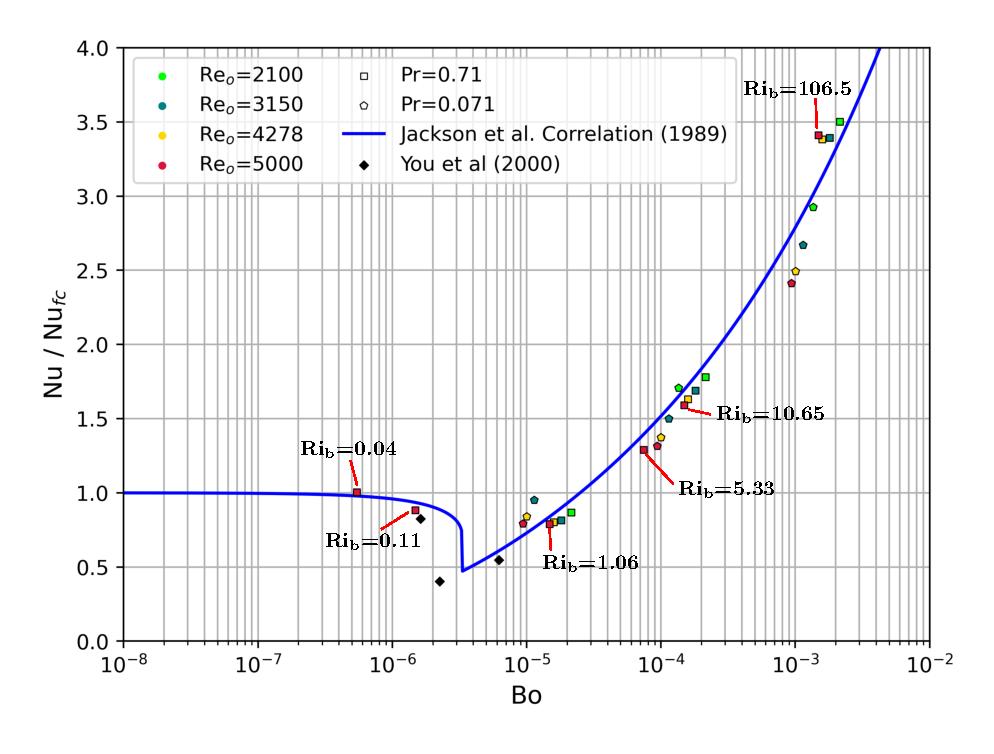
\includegraphics[width=0.65\textwidth]{figures/cap5/nusselt_corr/nu_corr.eps}
    \label{fig:nu_vs_bo}}
  \subfloat[]{
    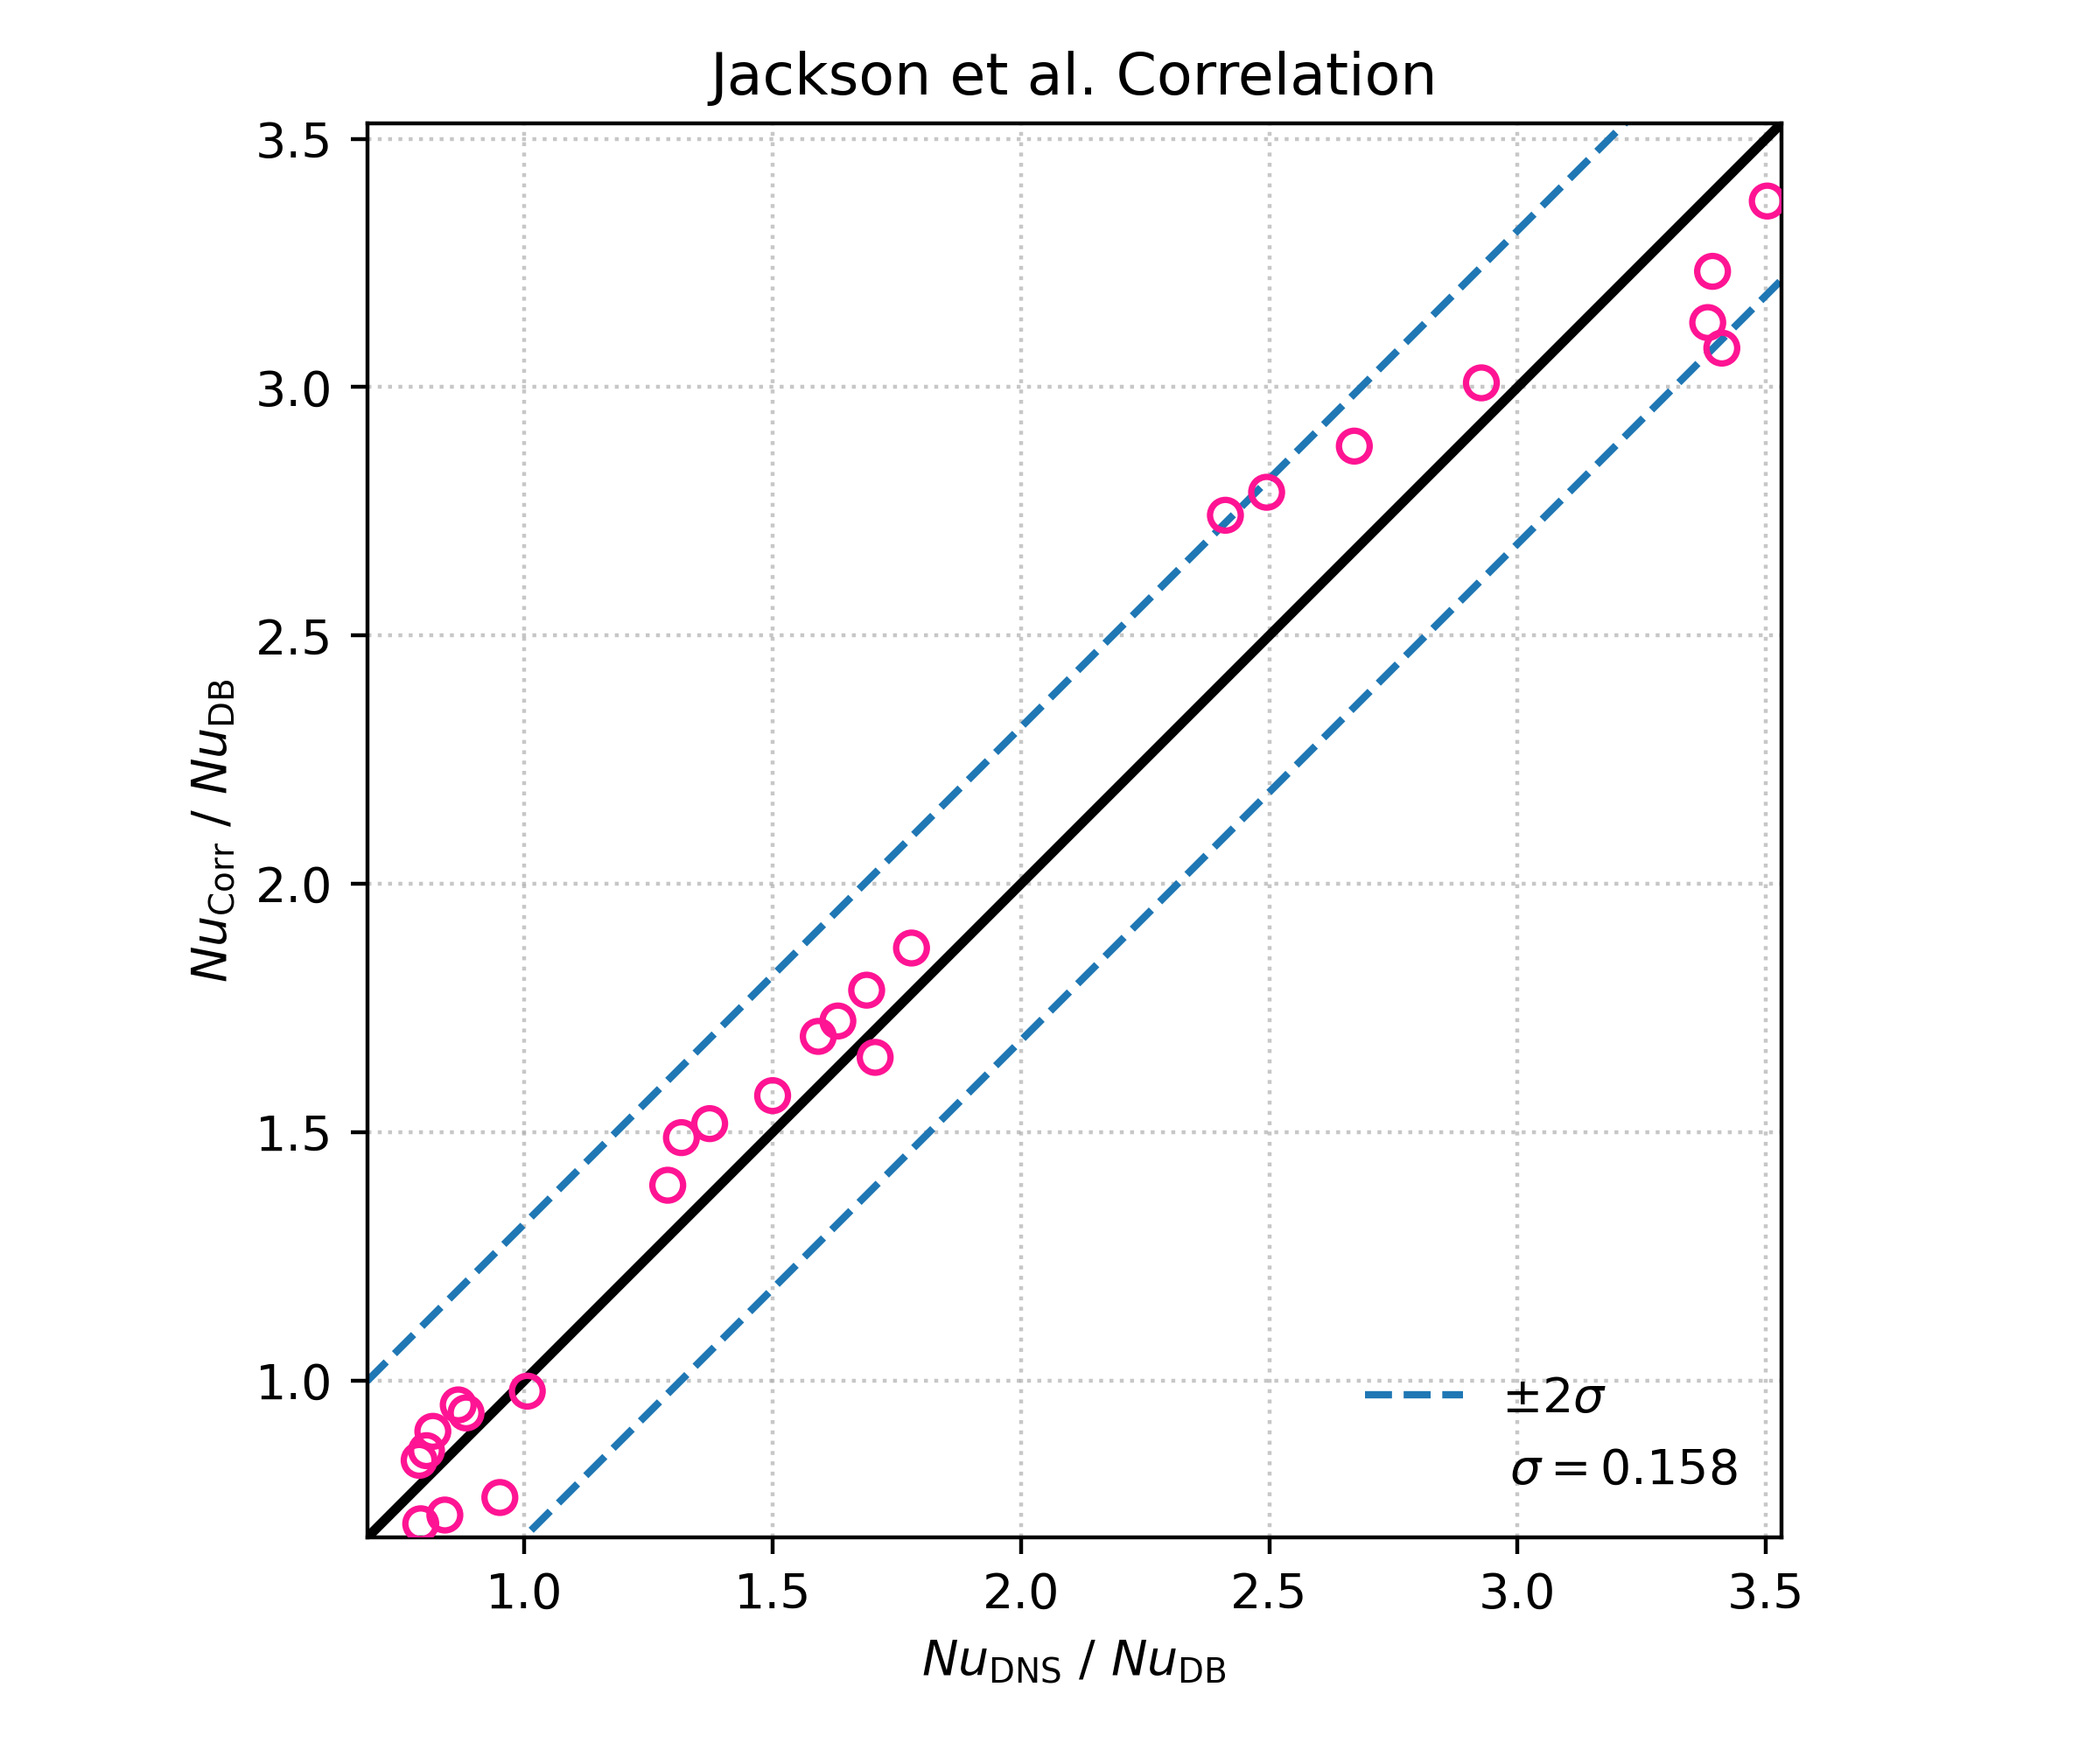
\includegraphics[width=0.33\textwidth]{figures/cap5/nusselt_corr/jackson_parity.png}
    \label{fig:parity}}
  \caption{\textbf{(a)} Número de Nusselt normalizado vs Bo; \textbf{(b)} paridad con la correlación de Jackson \textit{et al.} \cite{jackson1989studies}.}
  \label{fig:nusselt}
\end{figure}

En la definición de Nu, se puede apreciar su dependencia con el número de Reynolds y el número de Prandtl, y además, también es posible inferir su dependencia con la fuerza boyante. Para entender esto último, se retoman los conjuntos definidos en la sección \ref{sec:velo_temp}. En el primer conjunto la transferencia de calor por convección se deteriora, mientras que en el segundo conjunto dicha transferencia se recupera e incluso mejora respecto al caso de convección forzada pura (véanse los puntos representados con cuadrados rojos en la Figura \ref{fig:nu_vs_bo}). Estas observaciones, que no resultan intuitivas a primera vista, se esclarecen al examinar la Figura \ref{fig:uphi-Re5000-Pr071}, donde se representa el perfil medio $\langle u_x^{*}\theta^{*}\rangle$. El número de Nusselt es inversamente proporcional a $\langle\theta^{*}_b\rangle$ (ecuación \ref{eq:nu}), magnitud que depende del comportamiento de $\langle u_x^{*}\theta^{*}\rangle$. En consecuencia, con el aumento de la boyancia, la magnitud  $\langle u_x^{*}\theta^{*}\rangle$ tiende primero a aumentar (conjunto \textbf{I}) y luego a disminuir (conjunto \textbf{II}), lo que conduce a una reducción y posterior aumento de Nu, respectivamente. 

Se puede continuar la discusión sobre la variación de Nu con la fuerza boyante, agregando otros elementos de nuestras simulaciones. De acuerdo con el modelo de Prandtl \cite{Prandtl1942}, la transferencia de calor en flujos turbulentos se divide en dos mecanismos principales que actúan en serie: (i) conducción en la subcapa viscosa y (ii) el transporte de energía desde el borde de la capa viscosa al seno del fluido por el efecto difusivo de la turbulencia, siendo este último el efecto predominante \cite{aicher1997, hall1969laminarization}. Aicher y Martin \cite{aicher1997} sugieren que el transporte de energía es proporcional a la producción de turbulencia, que puede modelarse, a su vez, como proporcional al gradiente de velocidad \textit{streamwise} entre el seno del fluido y el borde de la capa viscosa. En base a nuestros resultados podemos cuantificar  cantidades relacionadas para evaluar el efecto de la turbulencia en la distribución de la energía térmica. 

\newpage

\begin{figure}[H] % usa [H] solo si necesitas anclarla y tienes \usepackage{float}
  \centering
  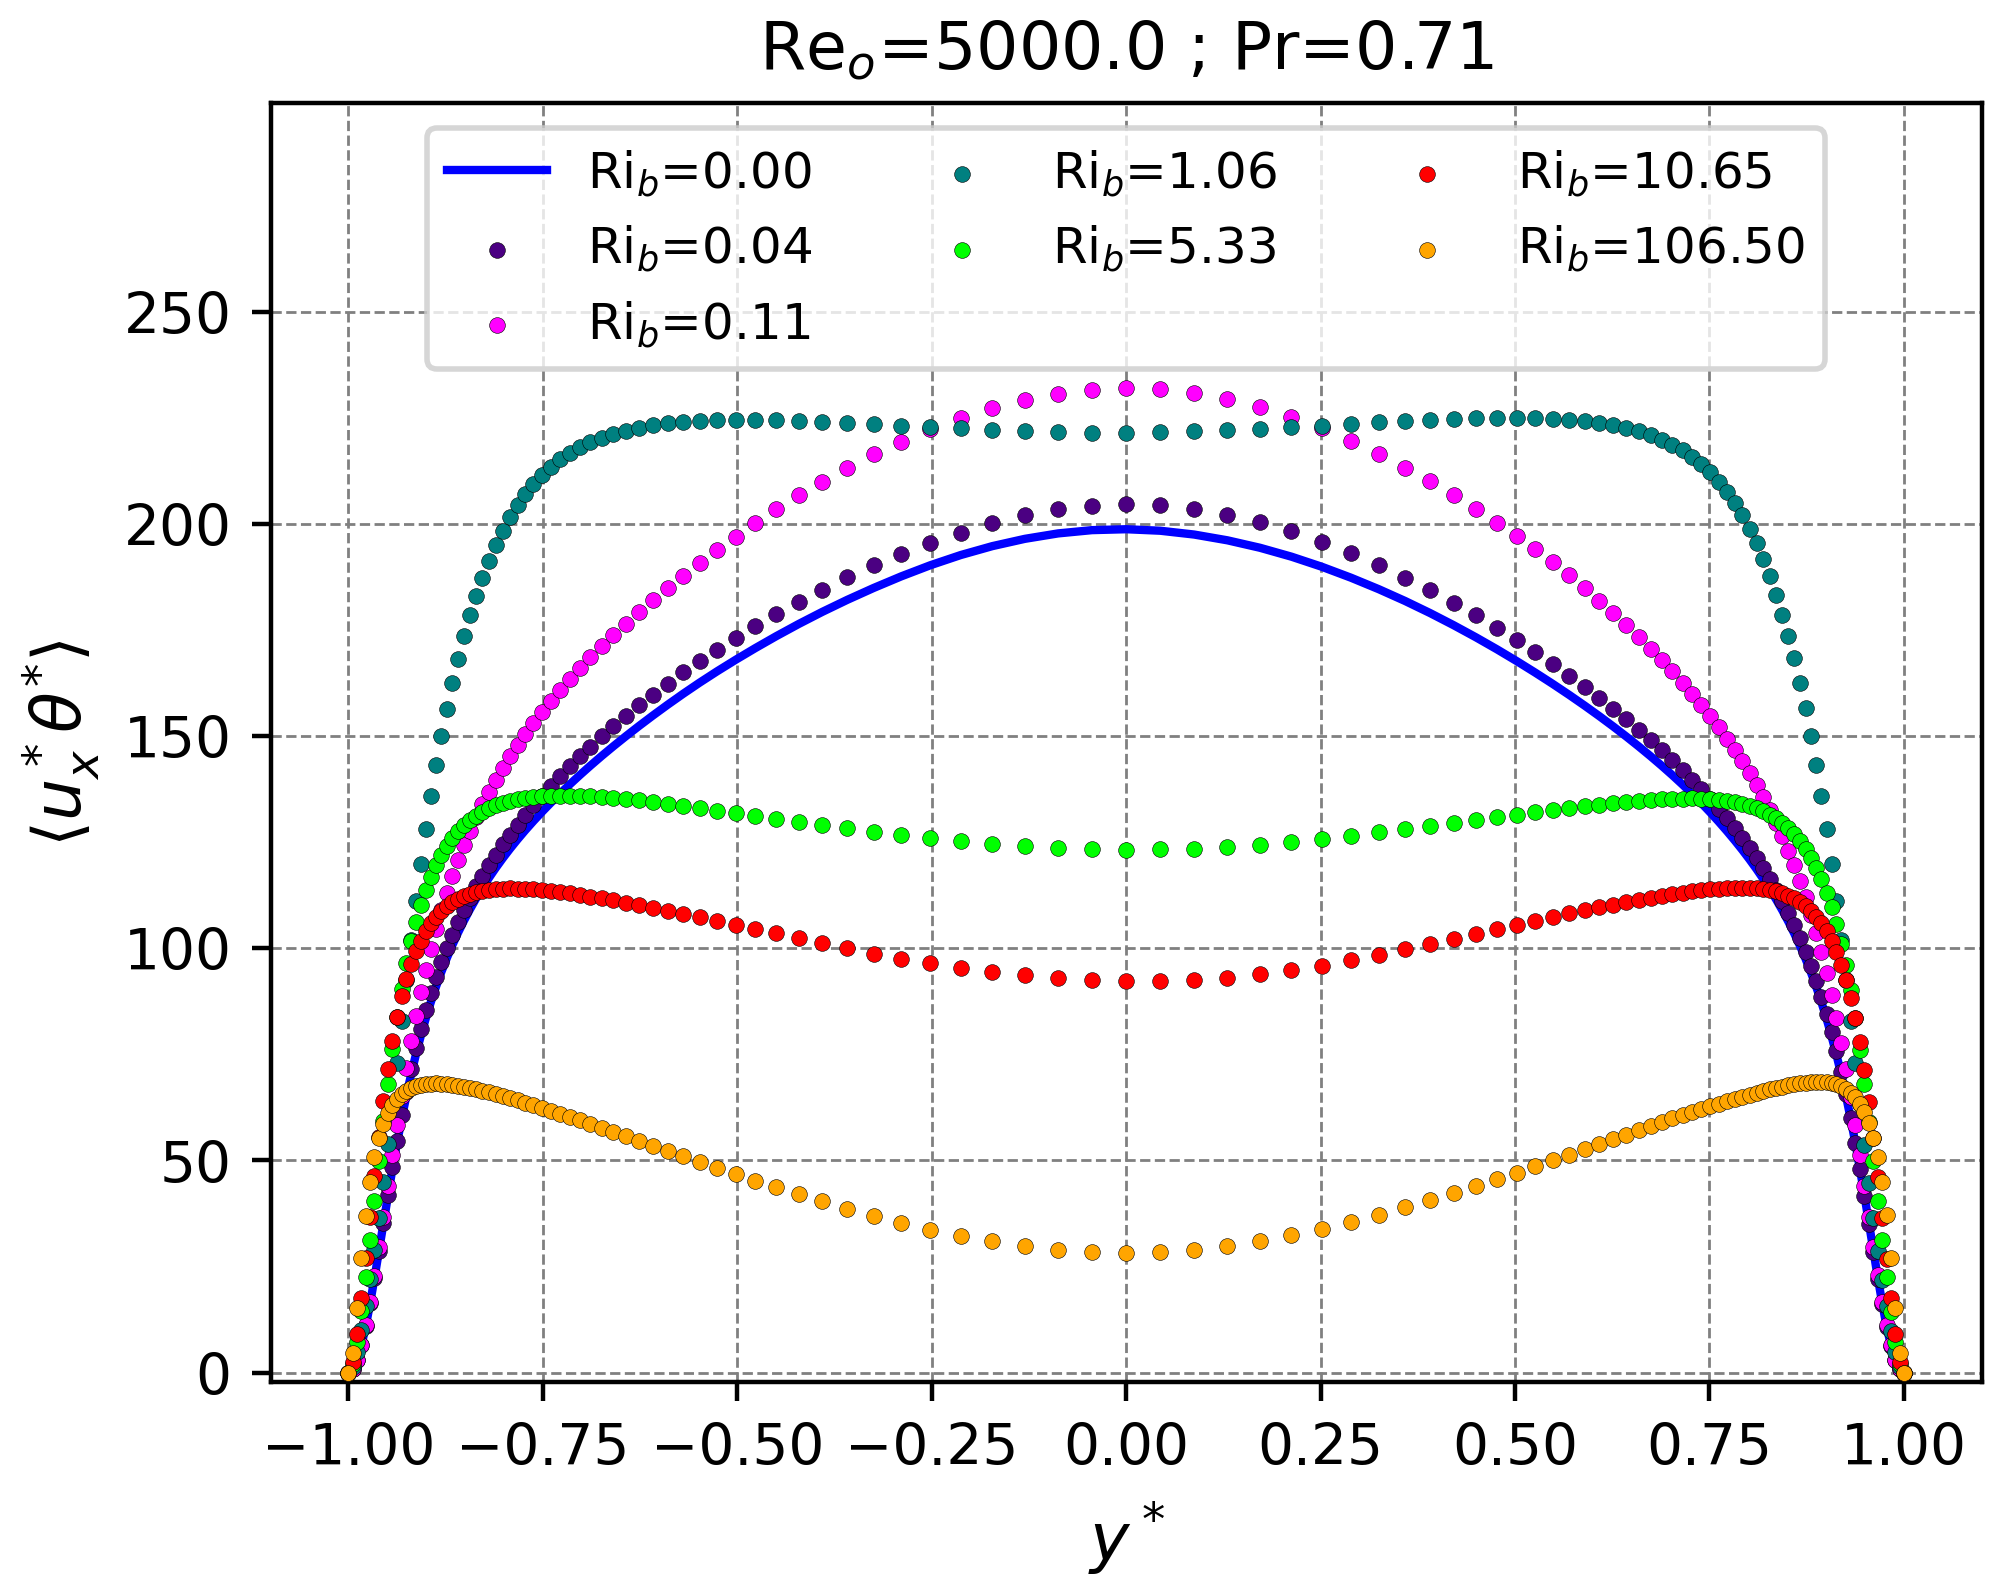
\includegraphics[width=0.6\textwidth]{figures/cap5/Re5000-Pr071/uxphi_profile.png}  
  \caption{Perfil de la magnitud media $\langle u^{*}_x\theta^{*}\rangle$.}
  \label{fig:uphi-Re5000-Pr071}
\end{figure}




En este contexto, la Figura \ref{fig:tke-prof} muestra el perfil de la energía cinética turbulenta para los casos simulados ($\text{Re}_o=5000$ y $\text{Pr}=0\text{.}71$) contemplando solo el semiancho del canal, esto es: $-1 \leqslant y^* \leqslant 0$. Si se considera el conjunto \textbf{I} de la Sección \ref{sec:velo_temp} ($0\text{.}04 \leq \text{Ri}_b \leq 1\text{.}06$), se observa que esta cantidad tiende a disminuir con el crecimiento de la boyancia; asimismo, el máximo tiende a desplazarse hacia la pared. Al contemplar el conjunto \textbf{II} ($\text{Ri}_b \geq 5\text{.}33$), el valor de TKE tiende a aumentar con la boyancia respecto al primer conjunto, y además, el máximo de las curvas tiende a desplazarse al centro del canal.

Por otro lado, la Figura \ref{fig:total_prod} representa la producción total de la TKE, esto es, la suma de la producción por cizalla $\mathcal{P}$ (\textit{Shear-Production}) y la producción por boyancia $\mathcal{B}$ (\textit{Buoyancy-Production}). Los términos $\mathcal{P}$ y $\mathcal{B}$ provienen del balance de energía cinética turbulenta $k$  (véase Apéndice \ref{apen:budgets}). En dicha figura, también se aprecia una disminución en la producción total con el aumento de la fuerza boyante para el conjunto \textbf{I}, mientras que los máximos de esta cantidad se trasladan hacia la pared. Por otro lado, los casos del conjunto \textbf{II} tienden a crecer con el aumento de la boyancia. Para todos los valores de $\text{Ri}_b$ de este conjunto, las cantidades experimentan dos máximos ``conectados'' por un valle. El primer máximo se mantiene muy próximo a la pared, prácticamente inmóvil con el aumento de la boyancia, y solo crece en amplitud. El segundo máximo, de menor amplitud que el primero, tiende a desplazarse hacia la pared mientras crece en amplitud con el aumento de la fuerza boyante.

Entonces, en virtud de lo discutido en los dos parrafos anteriores, es posible apreciar un rango de Ri$_b$, correspondiente al intervalo $10^{-6}$ $\lesssim$ Bo $\lesssim$ $3 \times 10^{-5}$ en la Figura \ref{fig:nu_vs_bo}, donde disminuye la producción total de turbulencia, y por lo tanto, el número de Nusselt. Asimismo, al examinar los perfiles de velocidad (Figura \ref{fig:ux-Re5000-Pr071}), su comportamiento resulta coherente con la hipótesis de Aicher \cite{aicher1997}. Esta, recuérdese, sugiere que la producción de turbulencia es proporcional a la diferencia de velocidades\footnote{Dicha diferencia puede interpretarse como proporcional a un gradiente de velocidades.} entre aquella en el borde de la capa viscosa (muy próxima a la pared) y aquella en el centro del canal. En el rango de Bo considerado, dicha diferencia (o gradiente) es nula o, en todo caso, muy pequeña.

Por lo tanto, si bien queda como trabajo futuro un análisis más exaustivo de los efectos de la fuerza boyante en el Nu, se encuentra una adecuada correspondencia entre los valores de TKE fuera de la capa viscosa, el comportamiento de los perfiles de velocidad y los valores del coeficiente de transferencia de calor.



\begin{figure}[H]
  \centering
  \subfloat[]{
    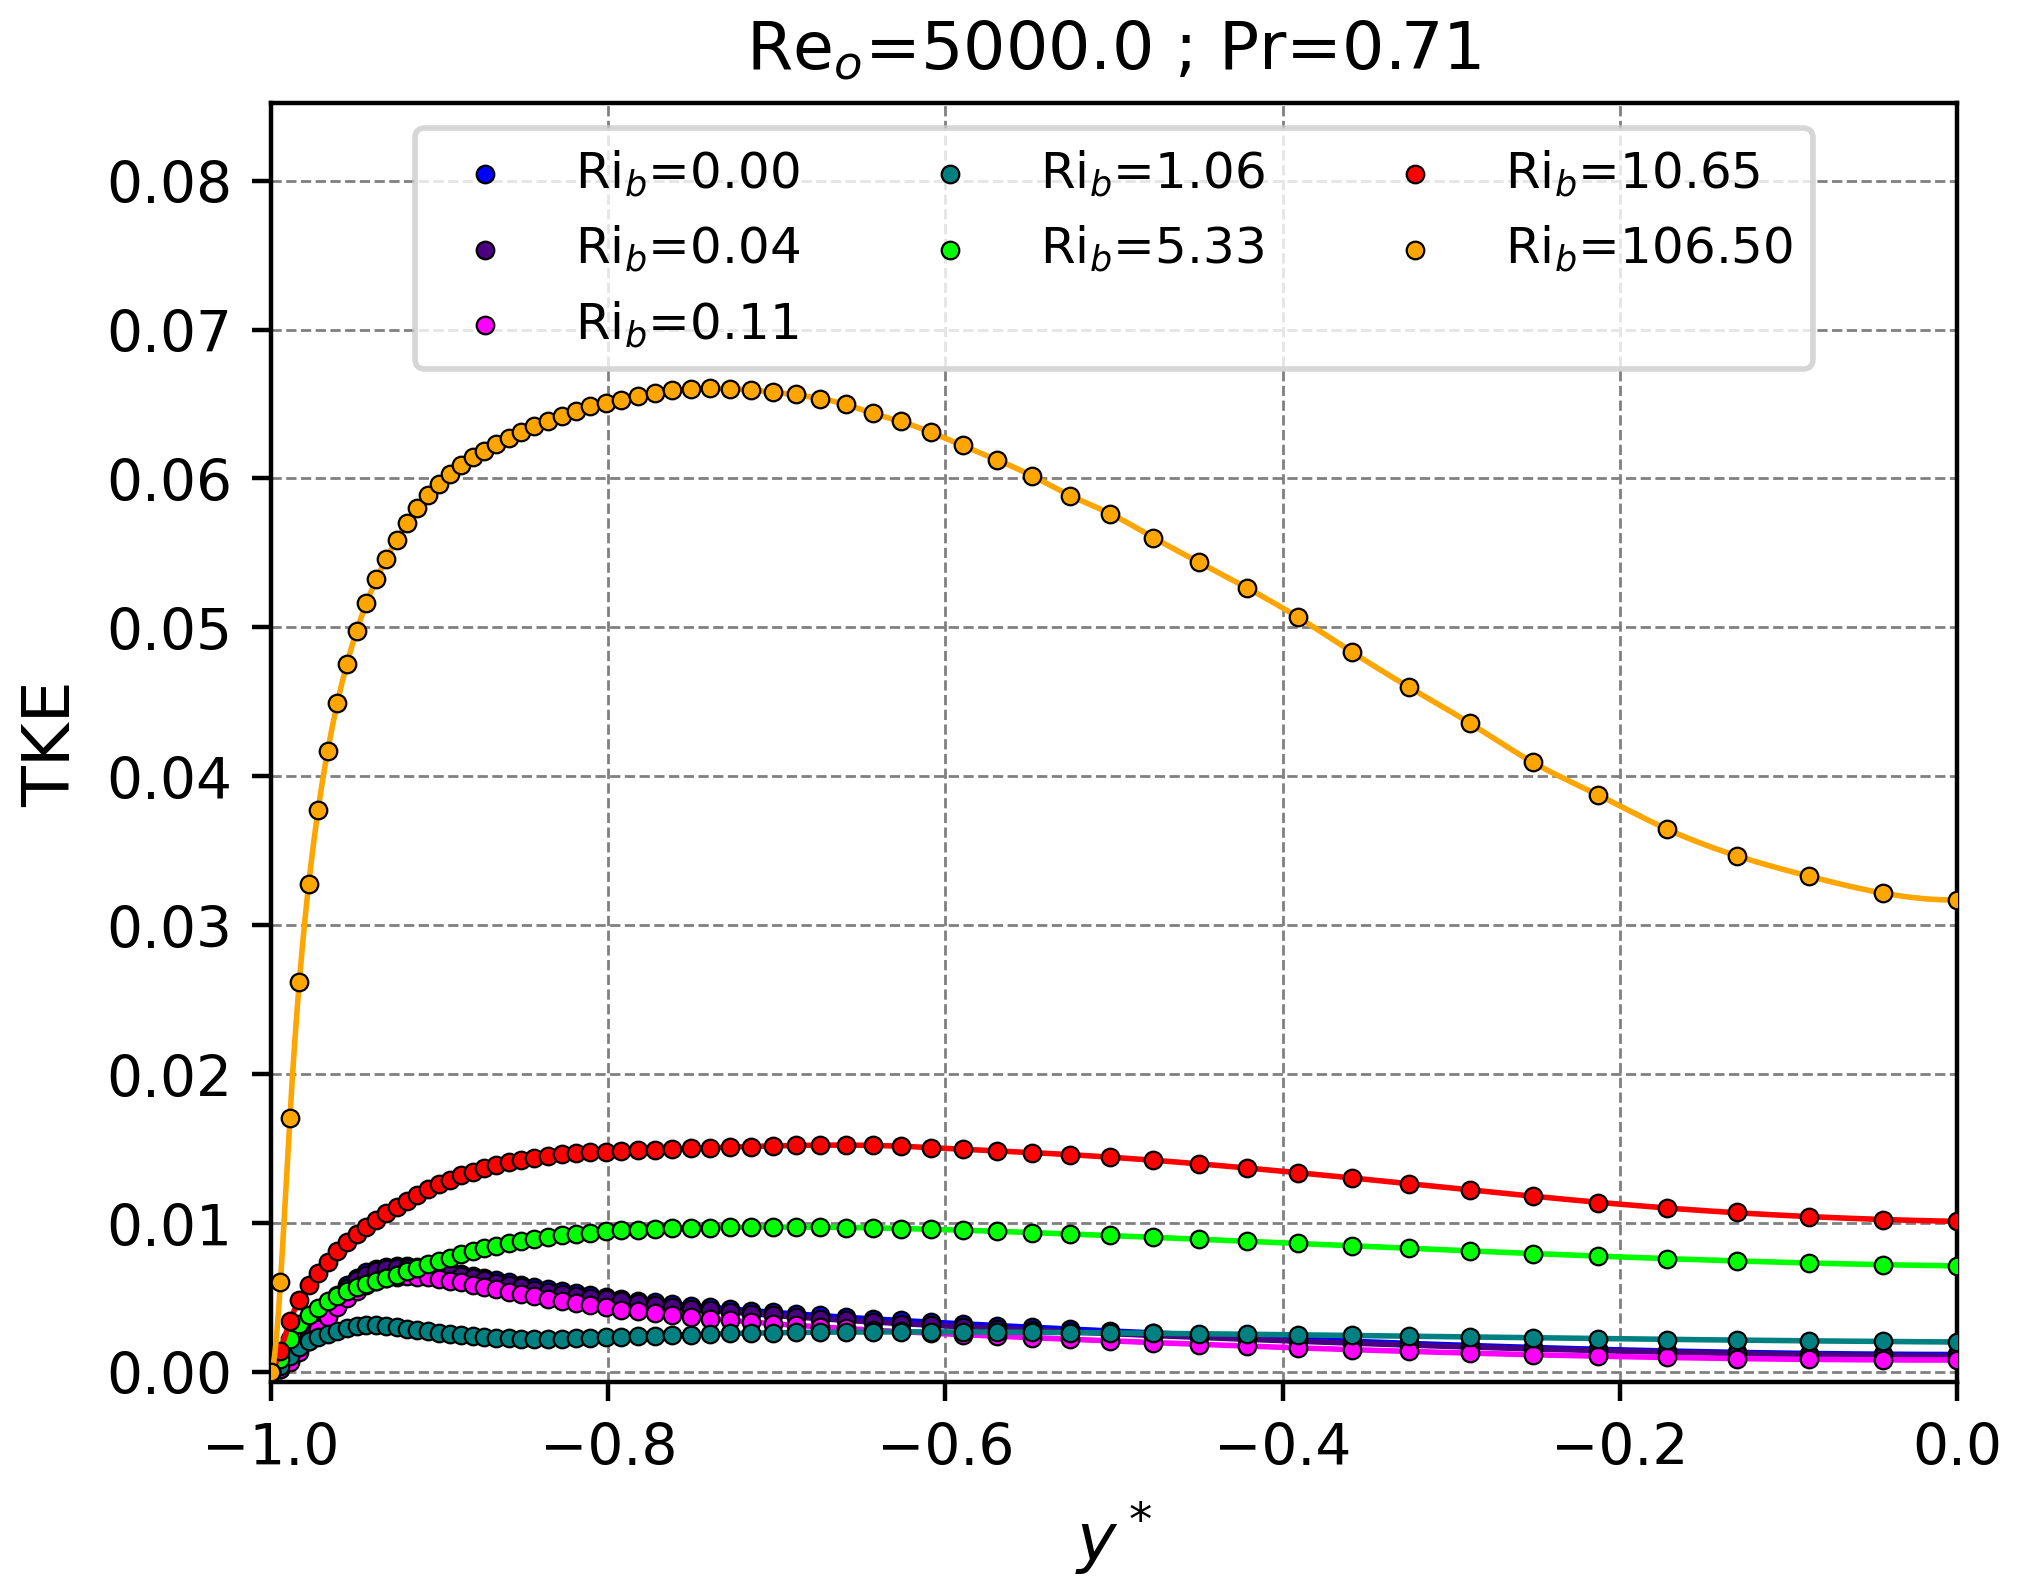
\includegraphics[width=0.46\textwidth]{figures/cap5/Re5000-Pr071/tke_profile.png}
    \label{fig:tke-prof}}
  \subfloat[]{
    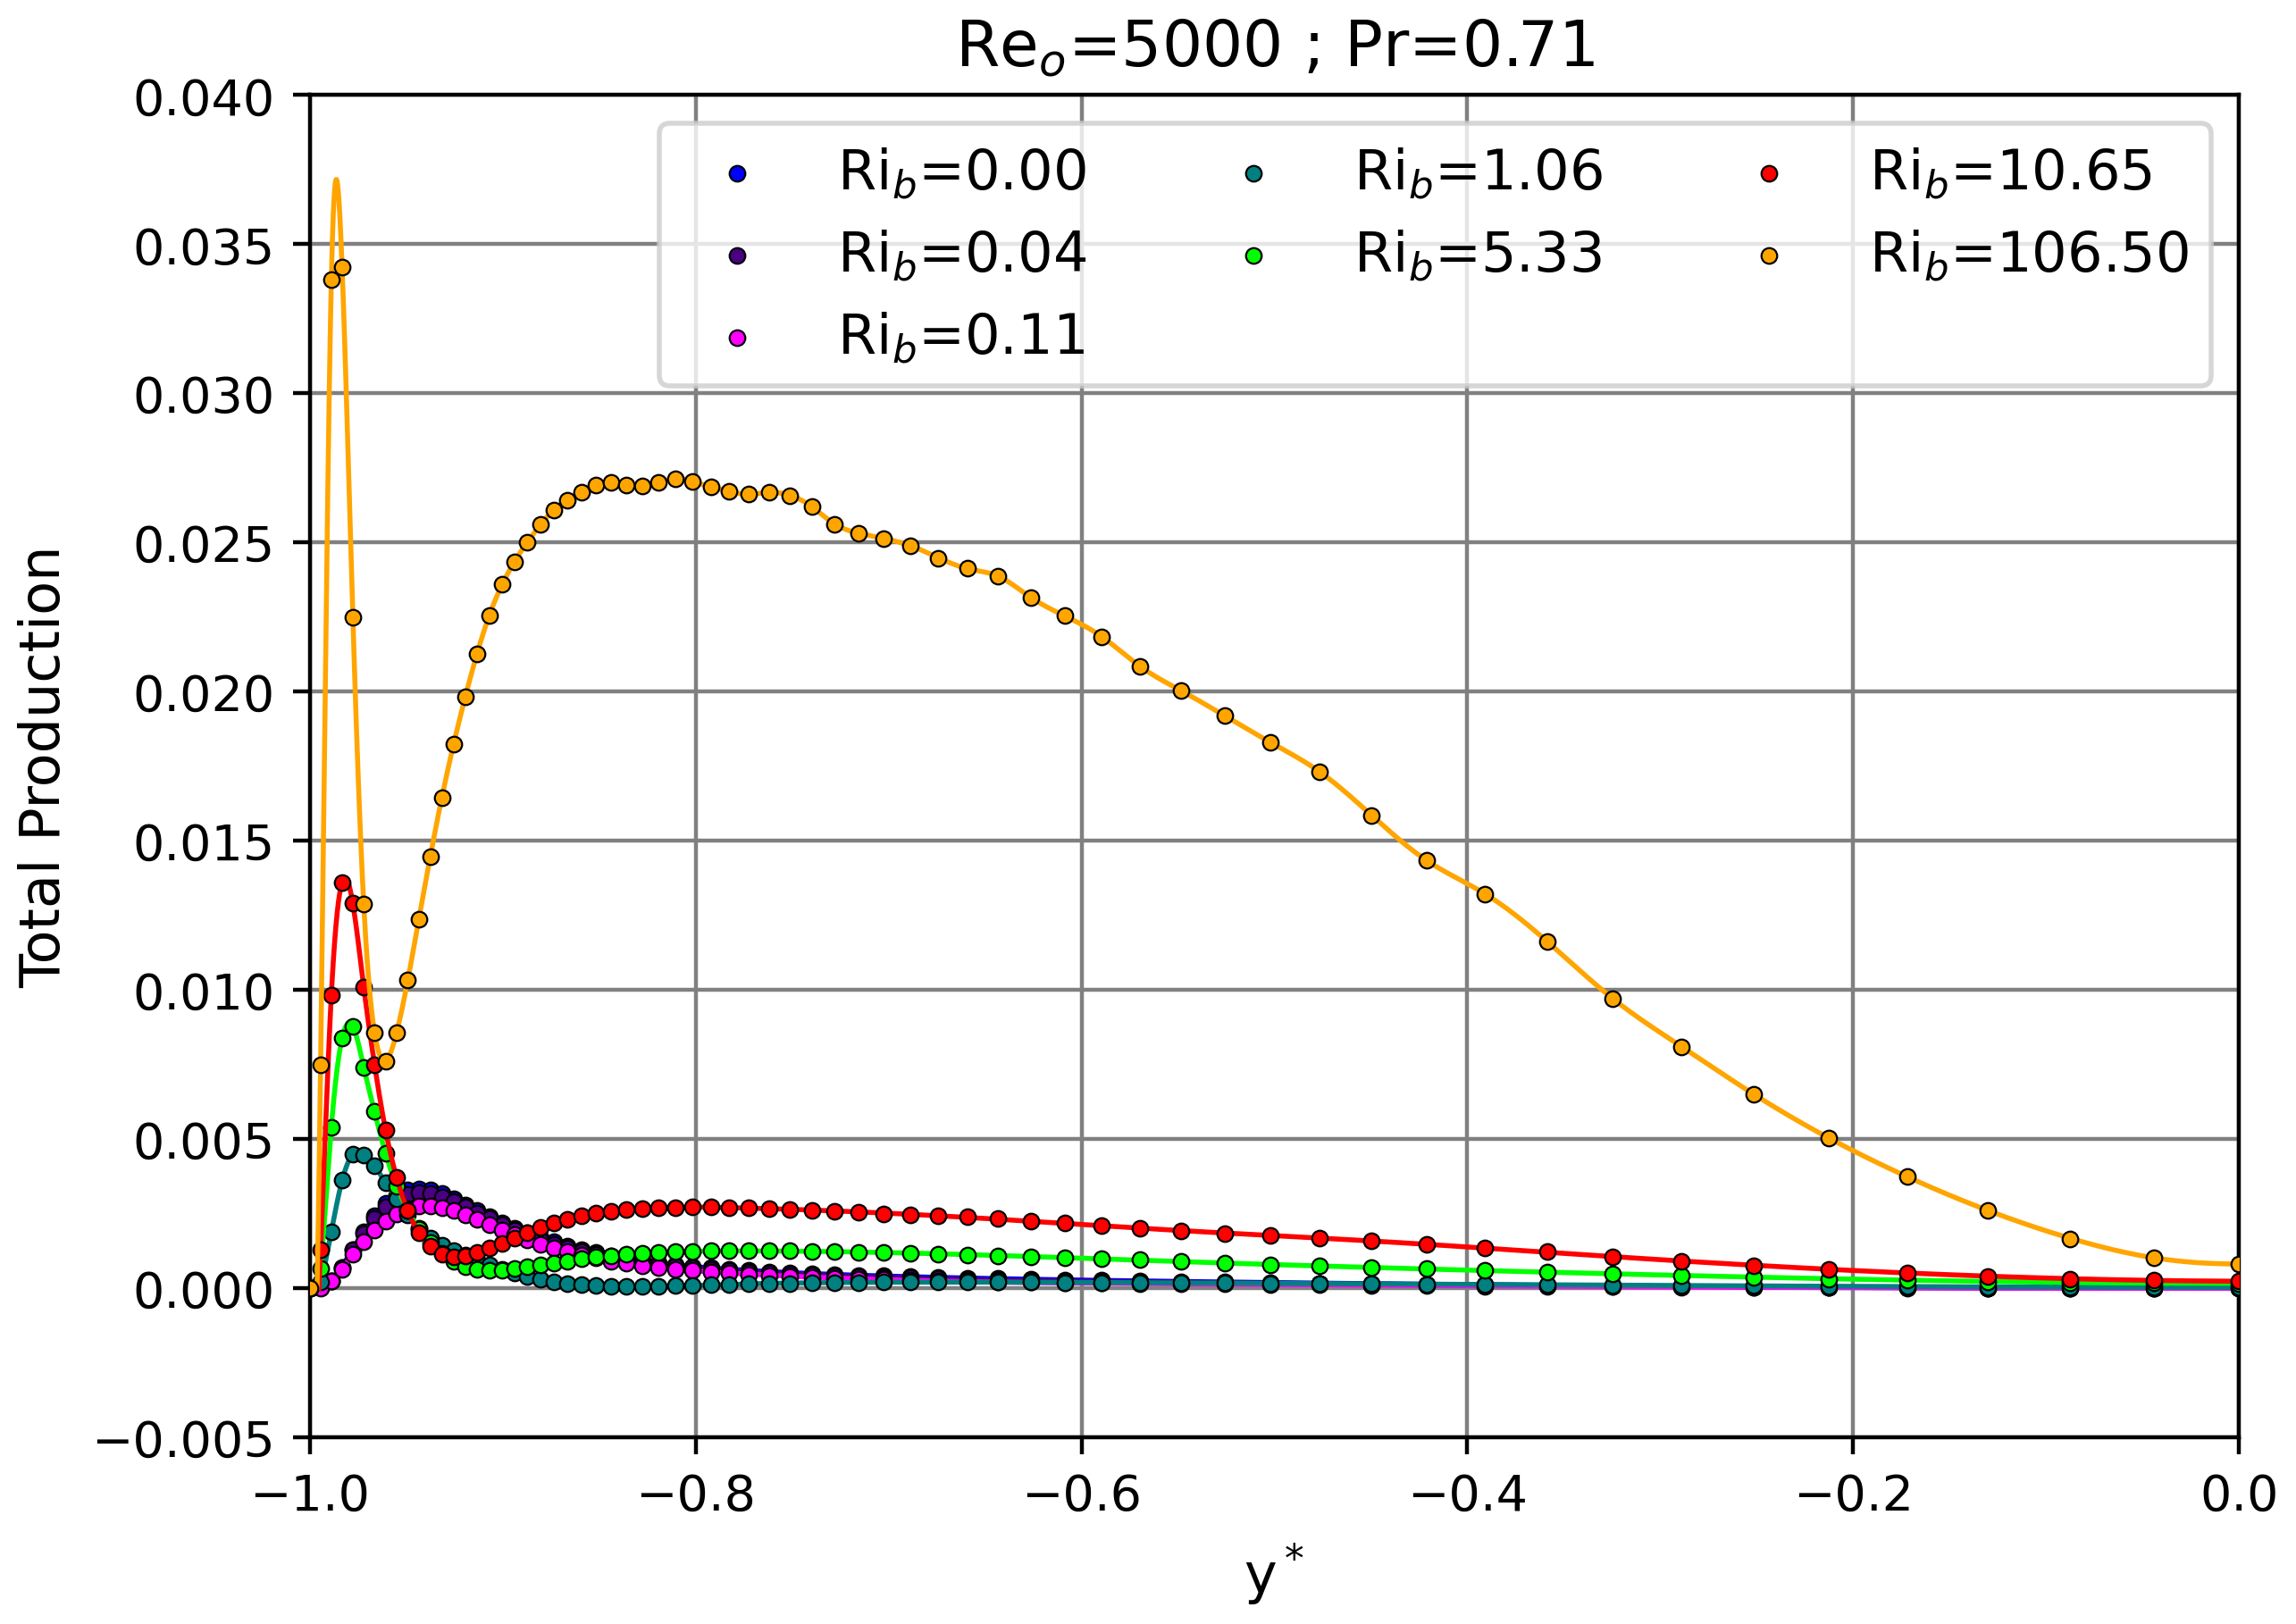
\includegraphics[width=0.51\textwidth]{figures/cap5/Re5000-Pr071-Ri1Em2_total_prod.png}
    \label{fig:total_prod}}
  \caption{\textbf{(a)} Perfil de la TKE; \textbf{(b)} producción total de turbulencia ($\mathcal{P} + \mathcal{B}$).}
  \label{fig:budgets_prod}
\end{figure}



\section{Factor de Fricción de Darcy}

En esta sección se analizan los resultados del coeficiente de fricción de Darcy. El mismo se define por la relación
\begin{equation}
f = 8 \frac{ \overline{\tau_w}}{\hspace{0.5mm} \rho \hspace{0.5mm} {U_b}^2 }  = \frac{18}{\text{Re}_o} \left.\frac{d \langle u^*_x \rangle}{dy}\right\vert_{wall} \text{.}
\label{eq:darcy}
\end{equation}
La Figura \ref{fig:darcy_vs_bo} recoge los valores de $f$ obtenidos en nuestras simulaciones DNS para una amplia gama de números de boyancia (ecuación \ref{eq:jackson_bo}). Se incluyen, además, datos experimentales de Parlatan et al. \cite{parlatan1996buoyancy} y de DNS de You et al. \cite{you2003direct}. Se observa una buena correspondencia entre los patrones de los tres conjuntos de datos. Por otro lado, la literatura ofrece pocas correlaciones para $f$ (o para el factor de Fanning) en flujo turbulento completamente desarrollado bajo régimen de convección mixta. Partiendo del planteo de Easby \cite{easby1978effect}, se propone una nueva forma funcional, dada por la ecuación \ref{eq:fcorr}, cuyos parámetros se ajustan con nuestros resultados (véase línea azul de la Figura \ref{fig:darcy_vs_bo}).
\begin{equation}
f_{corr} = C_1 + C_2 \hspace*{0.5mm} \text{Bo}^n
\label{eq:fcorr}
\end{equation}

\begin{small}
$$
C_1 = 0\text{.}031 \quad ; \quad C_2 = 10\text{.}031 \quad ; \quad n = 0\text{.}561
$$
\end{small}

La Figura \ref{fig:darcy_parity} muestra el gráfico de paridad $f_{\text{DNS}}$ frente a $f_{\text{corr}}$. La desviación estándar es $\sigma$=0.018 y el total de nuestros puntos se sitúa dentro de la banda de error, lo que confirma la fiabilidad de la correlación incluso al compararla con los datos de referencia externos.

\newpage

\begin{figure}[H]
  \centering
  \subfloat[]{
    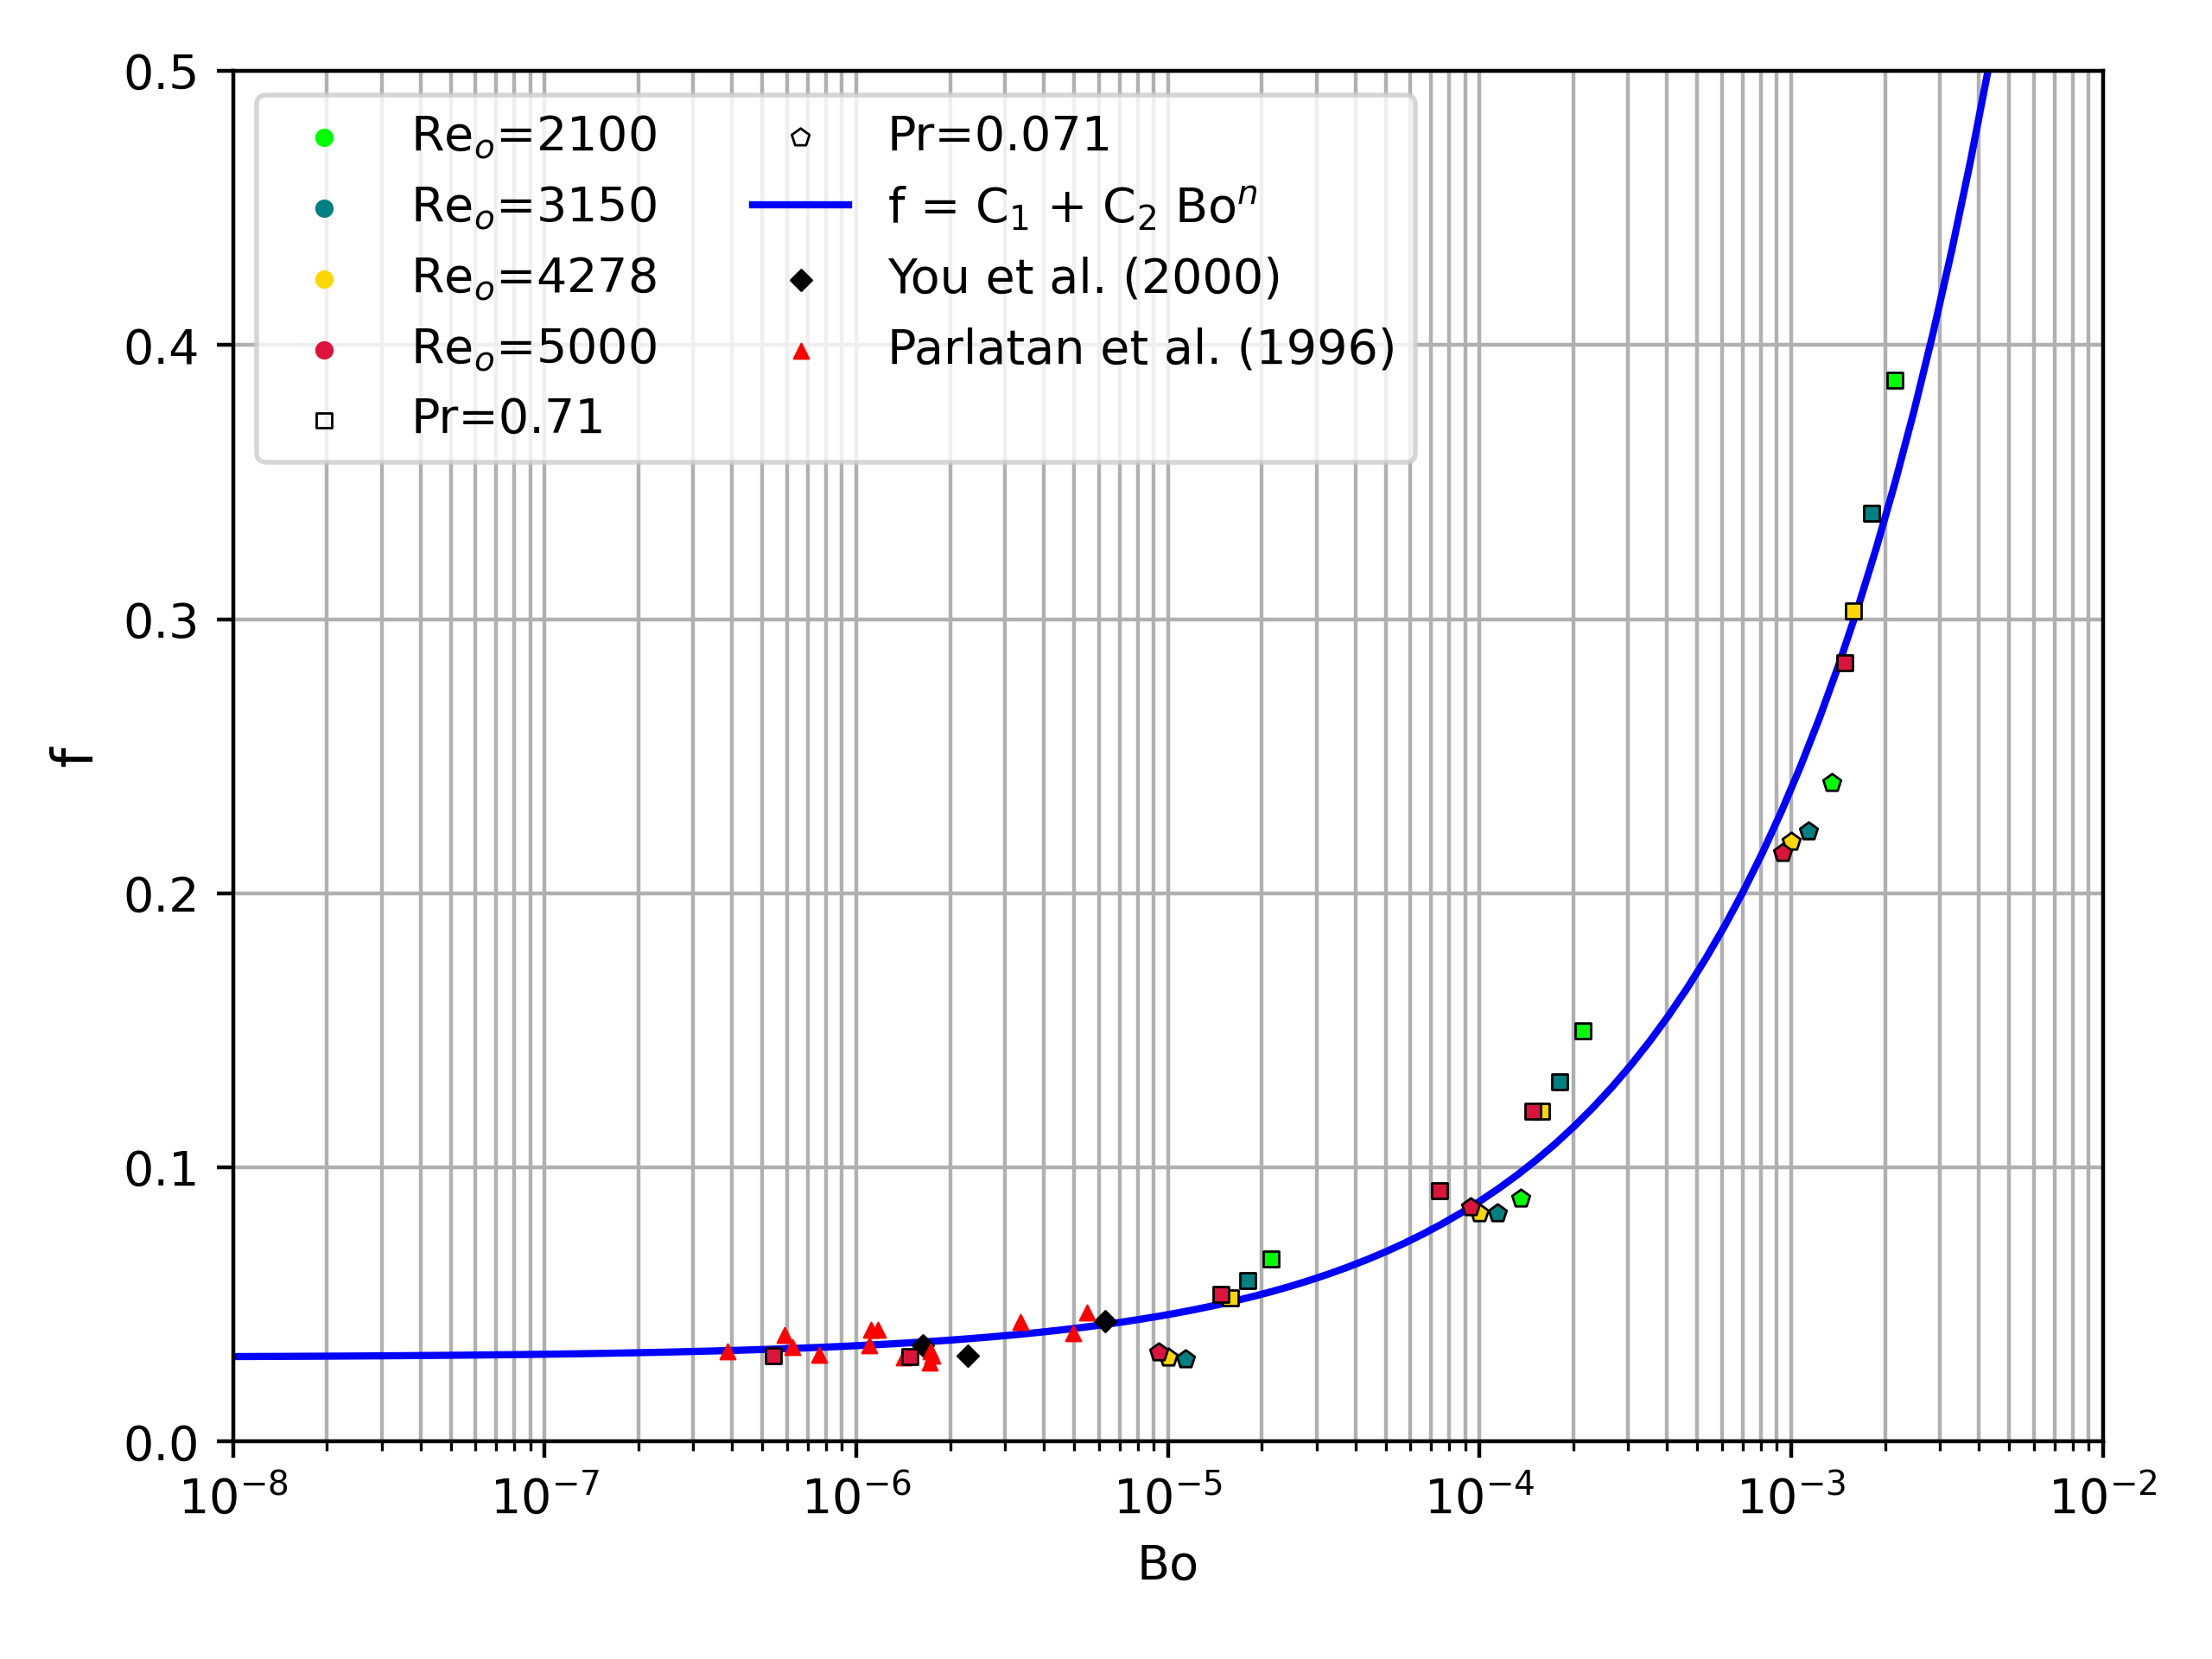
\includegraphics[width=0.55\textwidth]{figures/cap5/darcy/darcy_vs_Bo.png}
    \label{fig:darcy_vs_bo}}
  \subfloat[]{
    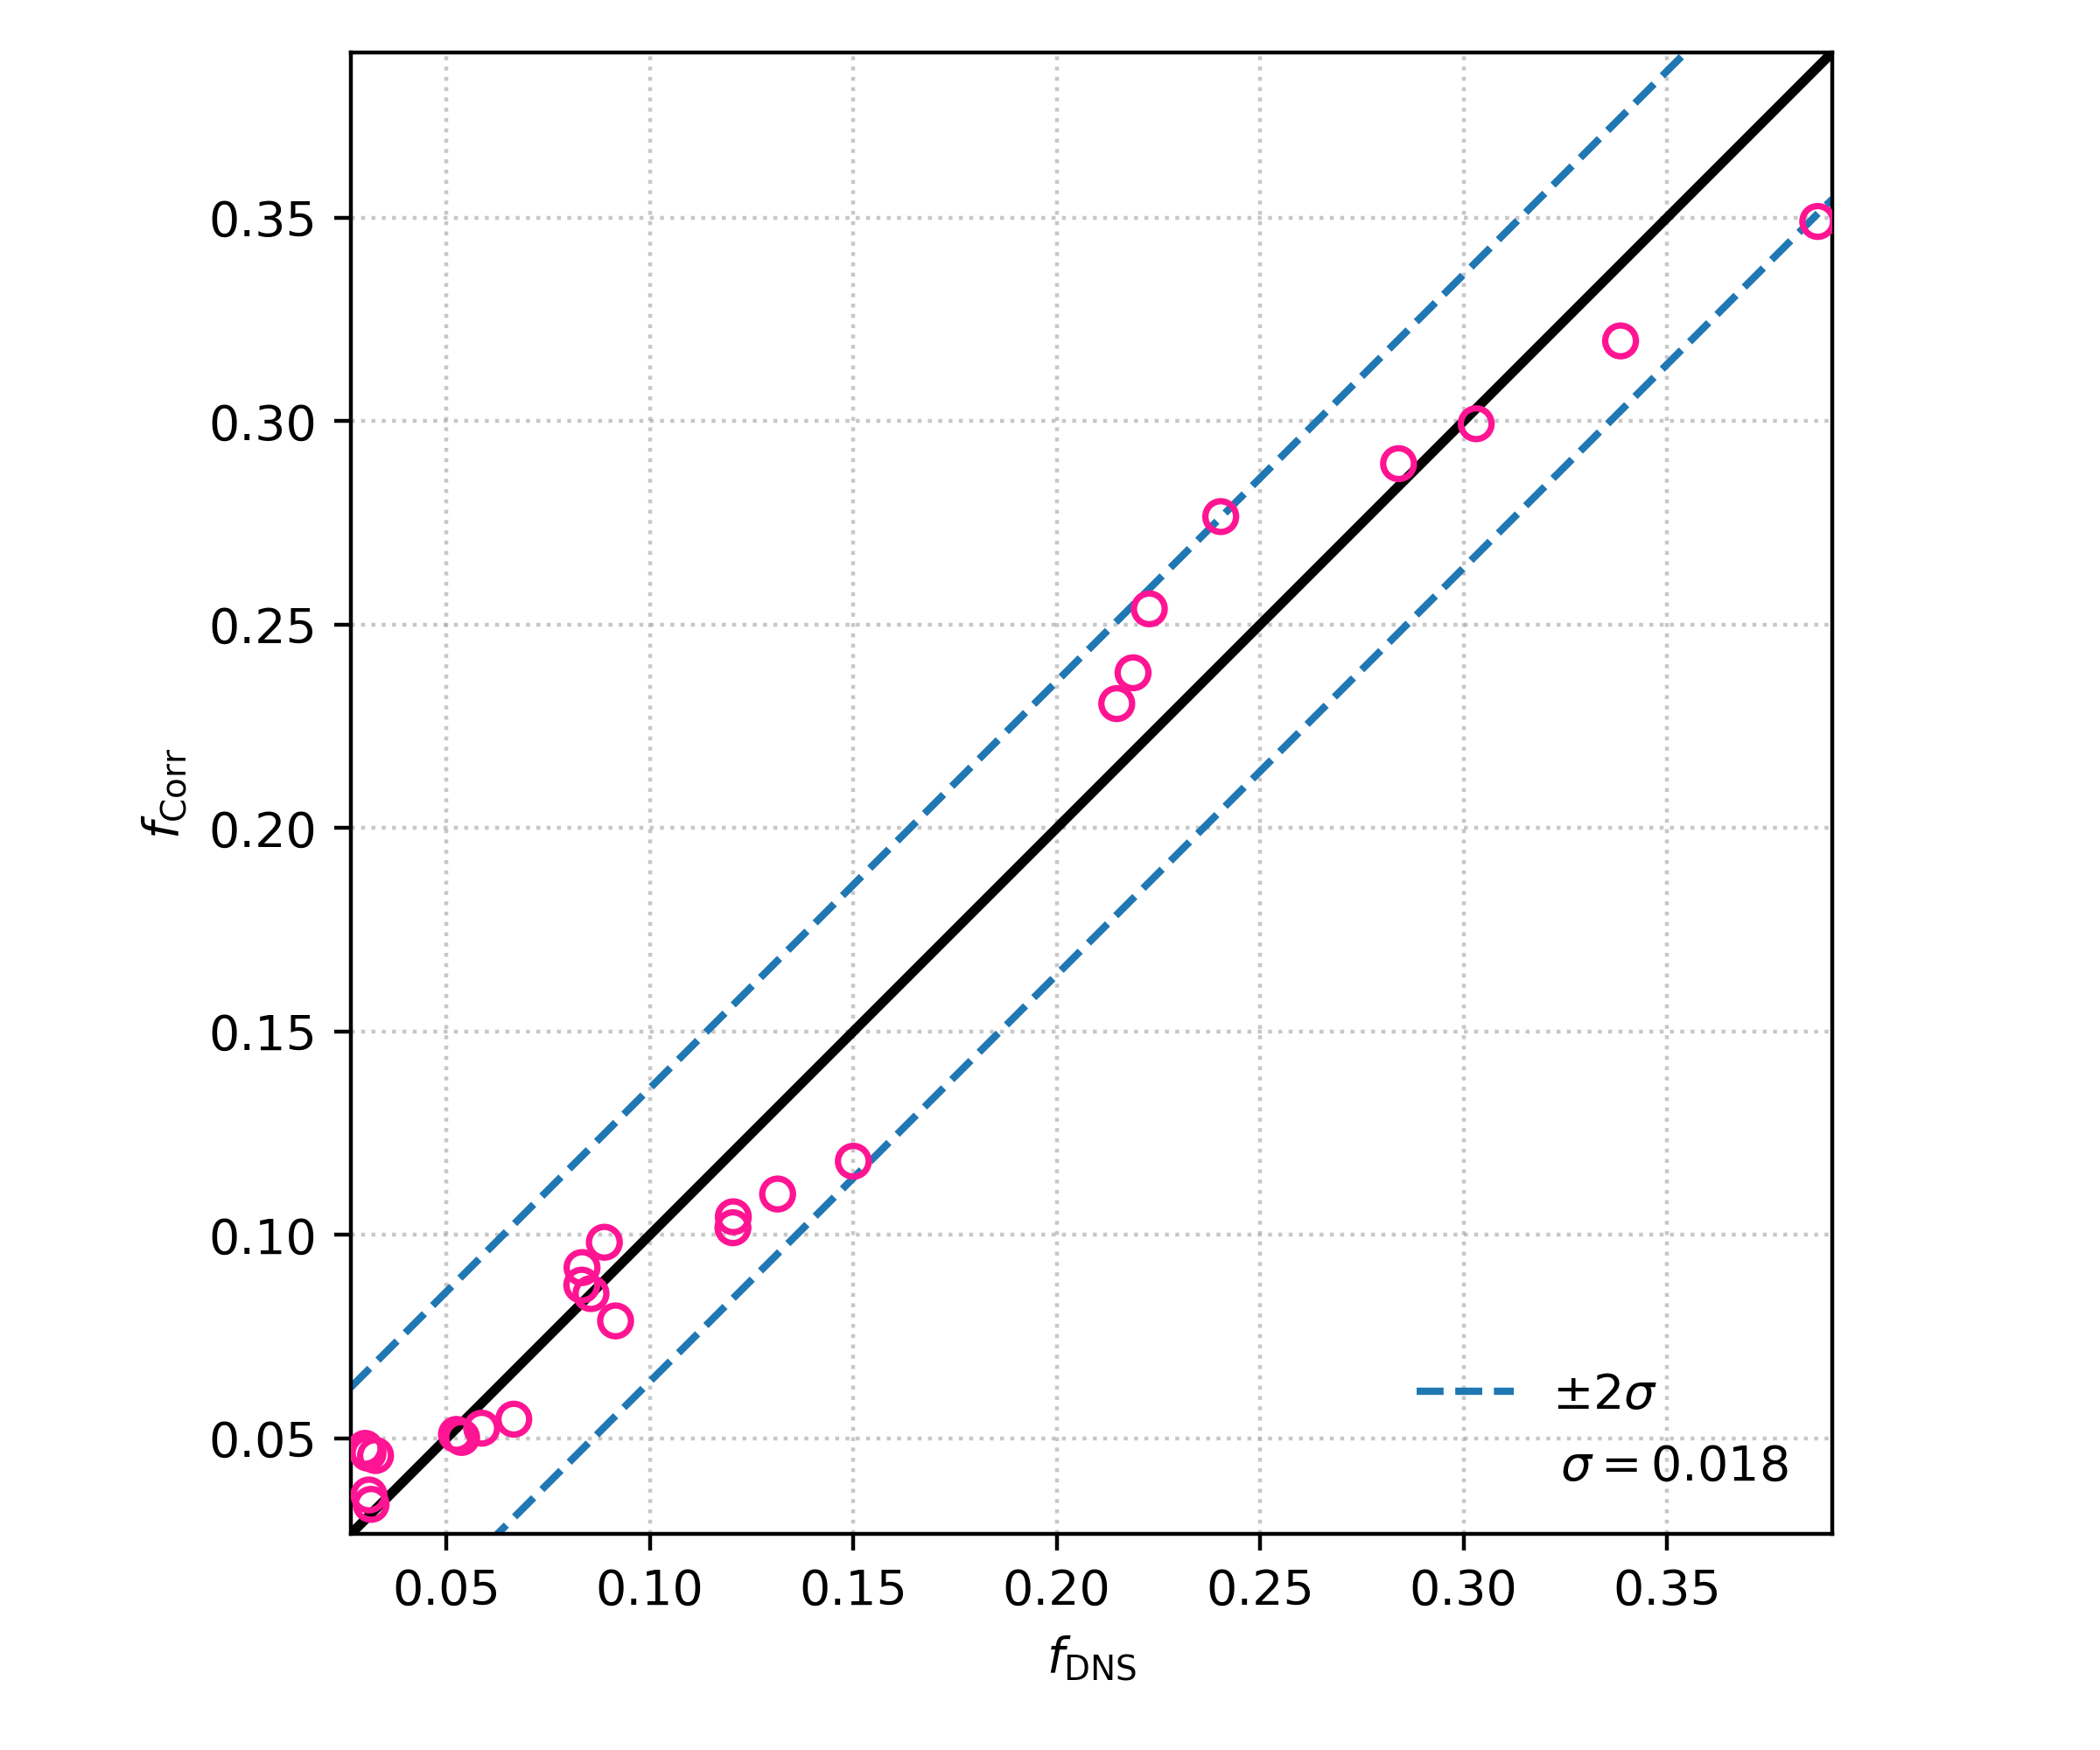
\includegraphics[width=0.44\textwidth]{figures/cap5/darcy/darcy_parity.png}
    \label{fig:darcy_parity}}
  \caption{\textbf{(a)} Coeficiente de fricción de Darcy vs Bo y \textbf{(b)} correlación propuesta; el ajuste reproduce los datos DNS con $\sigma$ = 0.018.}
  \label{fig:nusselt}
\end{figure}

El incremento de $f$ con la boyancia parece, a priori, contraintuitivo: al actuar la fuerza boyante en la misma dirección del flujo cabría esperar menores pérdidas de carga. Sin embargo, los perfiles de velocidad mostrados en la sección \ref{sec:velo_temp} evidencian que la boyancia acelera el fluido en las zonas próximas a la pared, lo que incrementa la pendiente $d \langle u^*_x \rangle / dx^*$ y, por ende, la tensión cortante media $\overline{\tau_w}$. Esta pérdida de carga por fricción se equilibra con la fuerza volumétrica producida por el cambio de densidad, y con la fuerza externa necesaria para mantener un caudal constante.


\newpage
\section{Sumario de los principales hallazgos}

\begin{itemize}

\item \textbf{Perfiles de velocidad:} la fuerza boyante genera perfiles tipo ``M'' y su incremento desplaza los máximos de $\langle u_x\rangle$ hacia la pared.

\item \textbf{Perfiles de temperatura:} Para flujos con $0 < \text{Ri}_b < 1$ los perfiles de temperatura adimensional se ubican por encima del caso puramente forzado. Para $\text{Ri}_b > 1$  la mezcla inducida por la flotación tiende a ``aplanar'' el perfil de la temperatura media adimensional.

\item \textbf{Efecto del Prandtl:} para Pr=0.071 la ley de pared de temperatura, $\langle\theta^*\rangle \simeq \text{Pr} \hspace{1mm} y^+$, se mantiene hasta $y^+ \approx 30$, mientras que para Pr=0.71 termina a $y^+ \approx 7$ mostrando la influencia de Pr en la capa conductiva.

\item \textbf{Degradación y mejora de Nu:} existe un intervalo $10^{-6} \lesssim \text{Bo} \lesssim 3 \times 10^{-5}$ donde Nu se reduce respecto al caso puramente forzado, y fuera de él, la transferencia se recupera y lo supera.

\item \textbf{Mecanismo energético:} la caída de Nu coincide con una disminución en la producción total de turbulencia que ocurre, principalmente, cerca de la pared.

\item \textbf{Factor de Darcy creciente:} pese a la asistencia de la boyancia, el gradiente de velocidad en la pared aumenta y eleva el factor de Darcy; la correlación $f_{\text{corr}}=C_1+C_2 Bo^n$ reproduce los datos simulados propios, y los datos de referencia, con buena fidelidad.

\end{itemize}

